\documentclass[12pt]{amsart}
\usepackage[T1]{fontenc}
\usepackage[utf8]{inputenc}

\usepackage[top=1.95cm, bottom=1.95cm, left=2.35cm, right=2.35cm]{geometry}

\usepackage{hyperref}
\usepackage{enumitem}
\usepackage{tcolorbox}
\usepackage{multicol}
\usepackage{fancyvrb}
\usepackage{amsmath}
\usepackage[french]{babel}
\usepackage[
    type={CC},
    modifier={by-nc-sa},
	version={4.0},
]{doclicense}
\usepackage{textcomp}
\usepackage{tcolorbox}
\usepackage{tnsmath}


\newtheorem{fact}{Fait}%[section]
\newtheorem*{theorem}{Théorème}
\newtheorem{example}{Exemple}[section]
\newtheorem{remark}{Remarque}[section]
\newtheorem*{proof*}{Preuve}

\setlength\parindent{0pt}


\DeclareMathOperator{\taille}{\text{\normalfont\texttt{taille}}}

\newcommand\sqseq[2]{\fbox{$#1$}_{\,\,#2}}

\newcommand\floor[1]{\left\lfloor #1 \right\rfloorx}


\DefineVerbatimEnvironment{rawcode}%
	{Verbatim}%
	{tabsize=4,%
	 frame=lines, framerule=0.3mm, framesep=2.5mm}



\begin{document}

\title{BROUILLON - Un simple (\!?) billard à deux bandes - Ajouter lien acvec PI : 3blue1brown galperin}
\author{Christophe BAL}
\date{25 Déc. 2018}

\maketitle

\begin{center}
	\itshape
	Document, avec son source \LaTeX, disponible sur la page

	\url{https://github.com/bc-writings/bc-public-docs/tree/main/drafts}.
\end{center}


\bigskip


\begin{center}
	\hrule\vspace{.3em}
	{
		\fontsize{1.35em}{1em}\selectfont
		\textbf{Mentions \og légales \fg}
	}

	\vspace{0.45em}
	\doclicenseThis
	\hrule
\end{center}



\setcounter{tocdepth}{2}
\tableofcontents



\section{Présentation du problème}

Voici une petite devinette bien sympathique.

\begin{enumerate}
    \item Dans des cases sont disposés à gauche uniquement des moutons noirs \textbf{N} et à droite que des blancs \textbf{B} avec une case vide entre chaque groupe. Voici un exemple.
    \centerit{\gameline{NNN.BBBB}}


    \item Les moutons noirs ne se déplacent que vers la droite, et les blancs uniquement vers la gauche. Aucun retour en arrière n'est possible !


    \item Pour avancer, un mouton ne peut faire que deux choses dans sa direction de déplacement.
    \begin{enumerate}
        \item Si la case vide est devant lui, un mouton peut avancer dans cette case.

        \item Un mouton peut sauter au-dessus d'un seul mouton d'une autre couleur pour arriver dans la case vide.
    \end{enumerate}
\end{enumerate}

\textbf{Question.} Peut-on faire passer tous les moutons blancs à gauche les uns à côté des autres, et tous les noirs à droite avec une case vide entre ces deux groupes de moutons ?


\bigskip


A titre d'exemple, considérons une partie avec la grille initiale suivante.

\centerit{\gameline{NN.BBB}}

Voici des mouvements possibles à partir de cette configuration.

\medskip

\begin{mvts}
    \item \gamelineplus*{NN.bBB}{Le \lmove{4}.}

    \medskip
    \item \gamelineplus*{Nnp.BB}{Le \rjump{2} au dessus d'un blanc.}

    \medskip
    \item \gamelineplus*{n.BuBB}{Le \rmove{1}}

    \medskip
    \item \gamelineplus*{.ubNBB}{Le \rjump{3} au dessus d'un noir.}

    \medskip
    \item \gamelineplus*{pn.NBB}{Le \rmove{2}}

    \medskip
    \item \gamelineplus*{B.uNBB}{Plus aucun mouvement n'est possible. Partie perdue !}
\end{mvts}

Si le coeur vous en dit, n'hésitez pas à tenter de résoudre cette devinette en prenant par exemple $3$ moutons noirs et $3$ blancs.



\section{Rechercher et conjecturer}

Dans un repère orthogonal, donnons nous la parabole $\setgeo{P} : y = x^2$ . Plaçons-y les points $A$ , $B$ et $S$ d'abscisses respectives $a$ , $b$ et  $s = a + b$ .
Observez
\footnote{
	Le lieu de téléchargement de ce document contient un fichier GeoGebra \texttt{base-tool.ggb} manipulable dynamiquement pour vérifier combien il est aisé de conjecturer quelque chose.
}
les trois cas ci-dessous et essayez de conjecturer quelque chose \emph{(la réponse est donnée dans la page suivante)}
\footnote{
	On peut géométriquement additionner modulo $2 \pi$ sur un cercle.
	Or $x^2 - y^2$ et $x^2 - y$ sont des formes quadratiques avec des propriétés géométriques communes.
	C'est là l'origine de la recherche proposée ici.
}.


\vspace{2.5em}

\begin{multicols}{2}
	\center
	\footnotesize
	\itshape
	
	\fbox{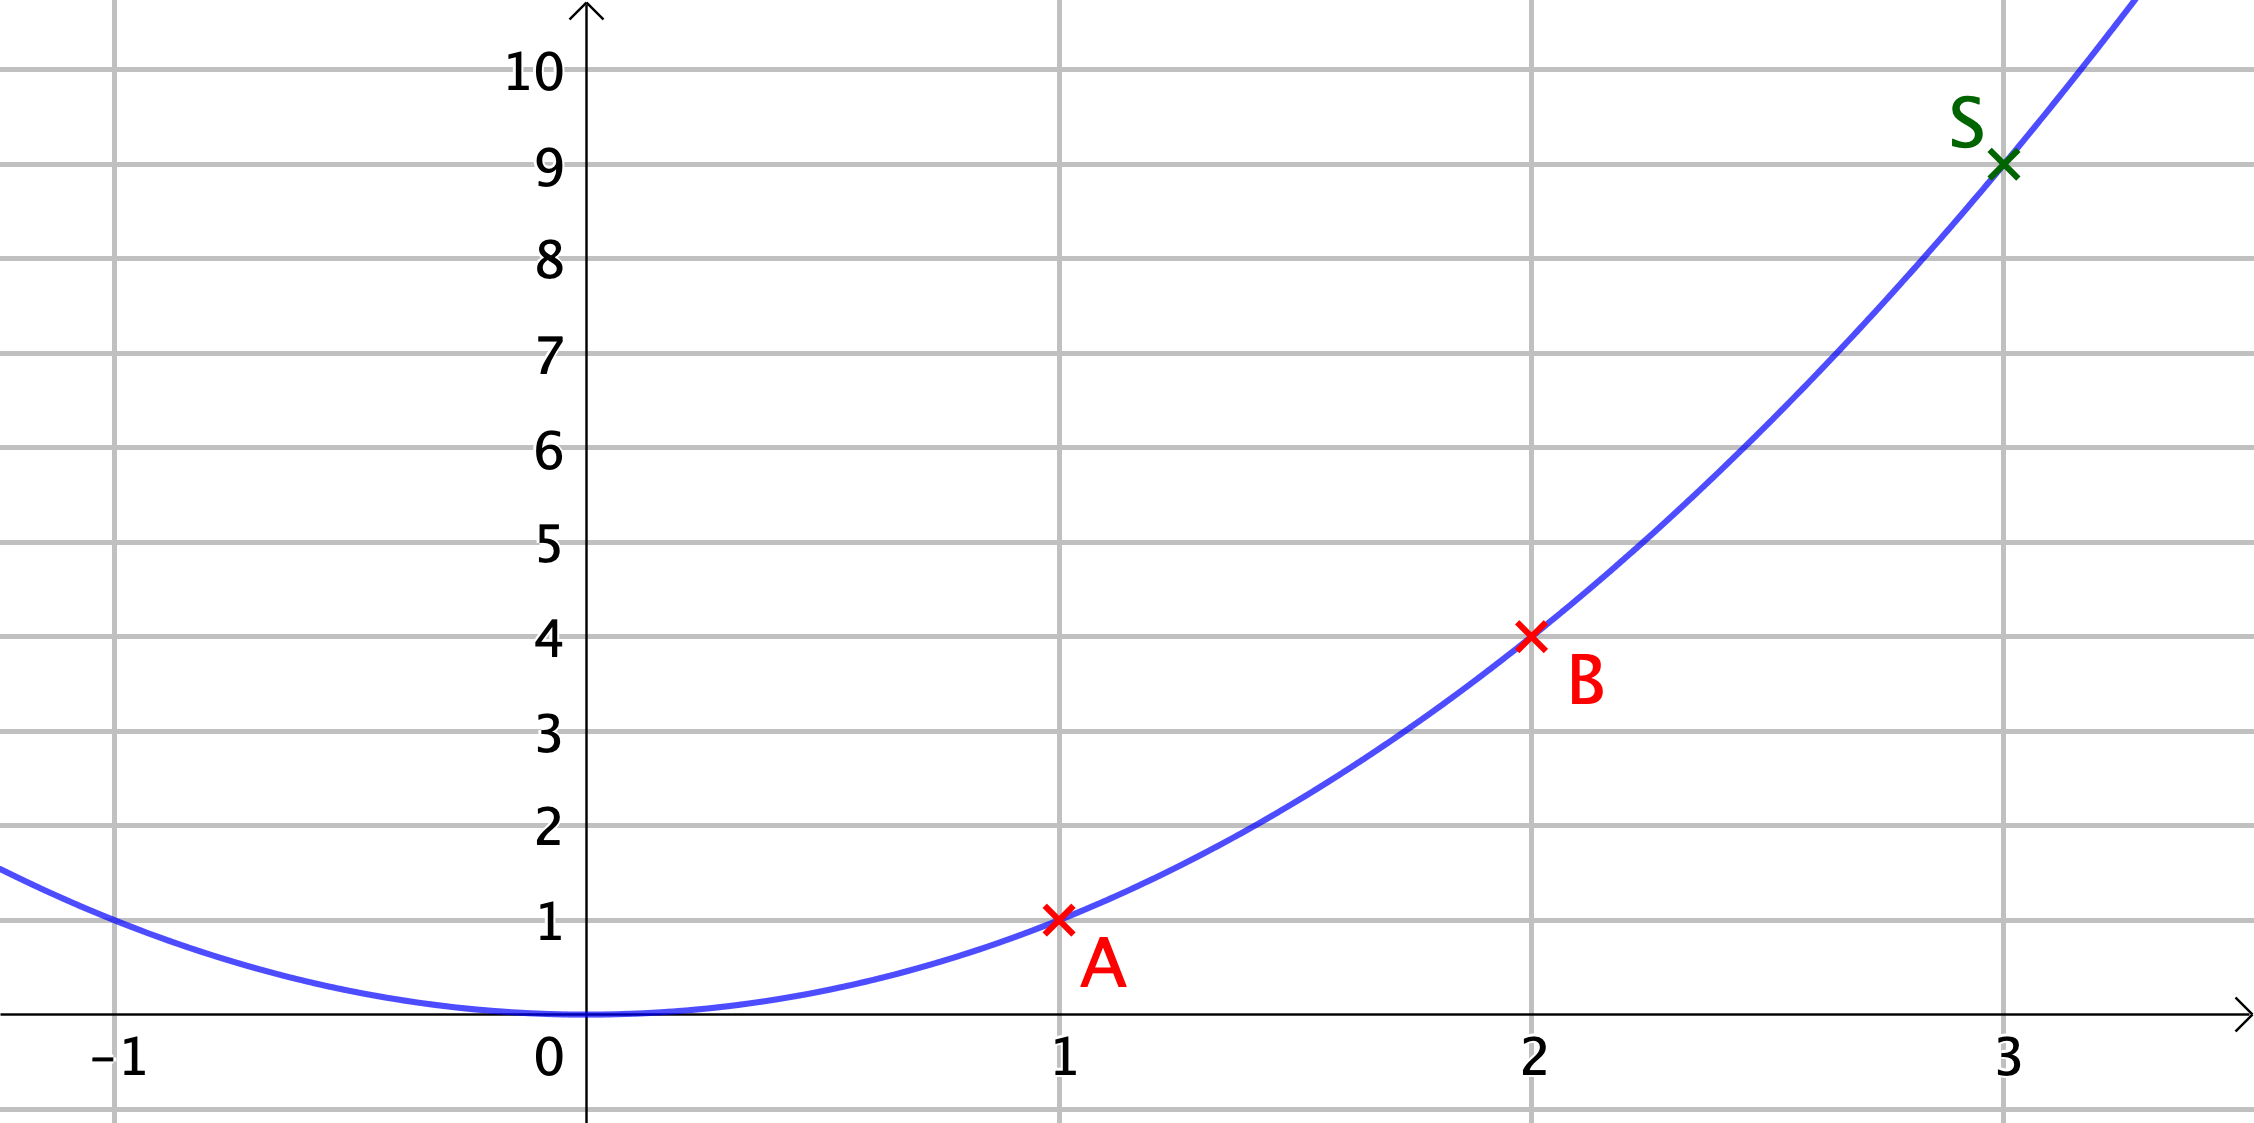
\includegraphics[scale = .8]{addition-on-parabolas/conjecture/a-and-b-positive.png}}
	
	\smallskip
	Cas où $a > 0$ et $b > 0$

	\columnbreak
	
	\fbox{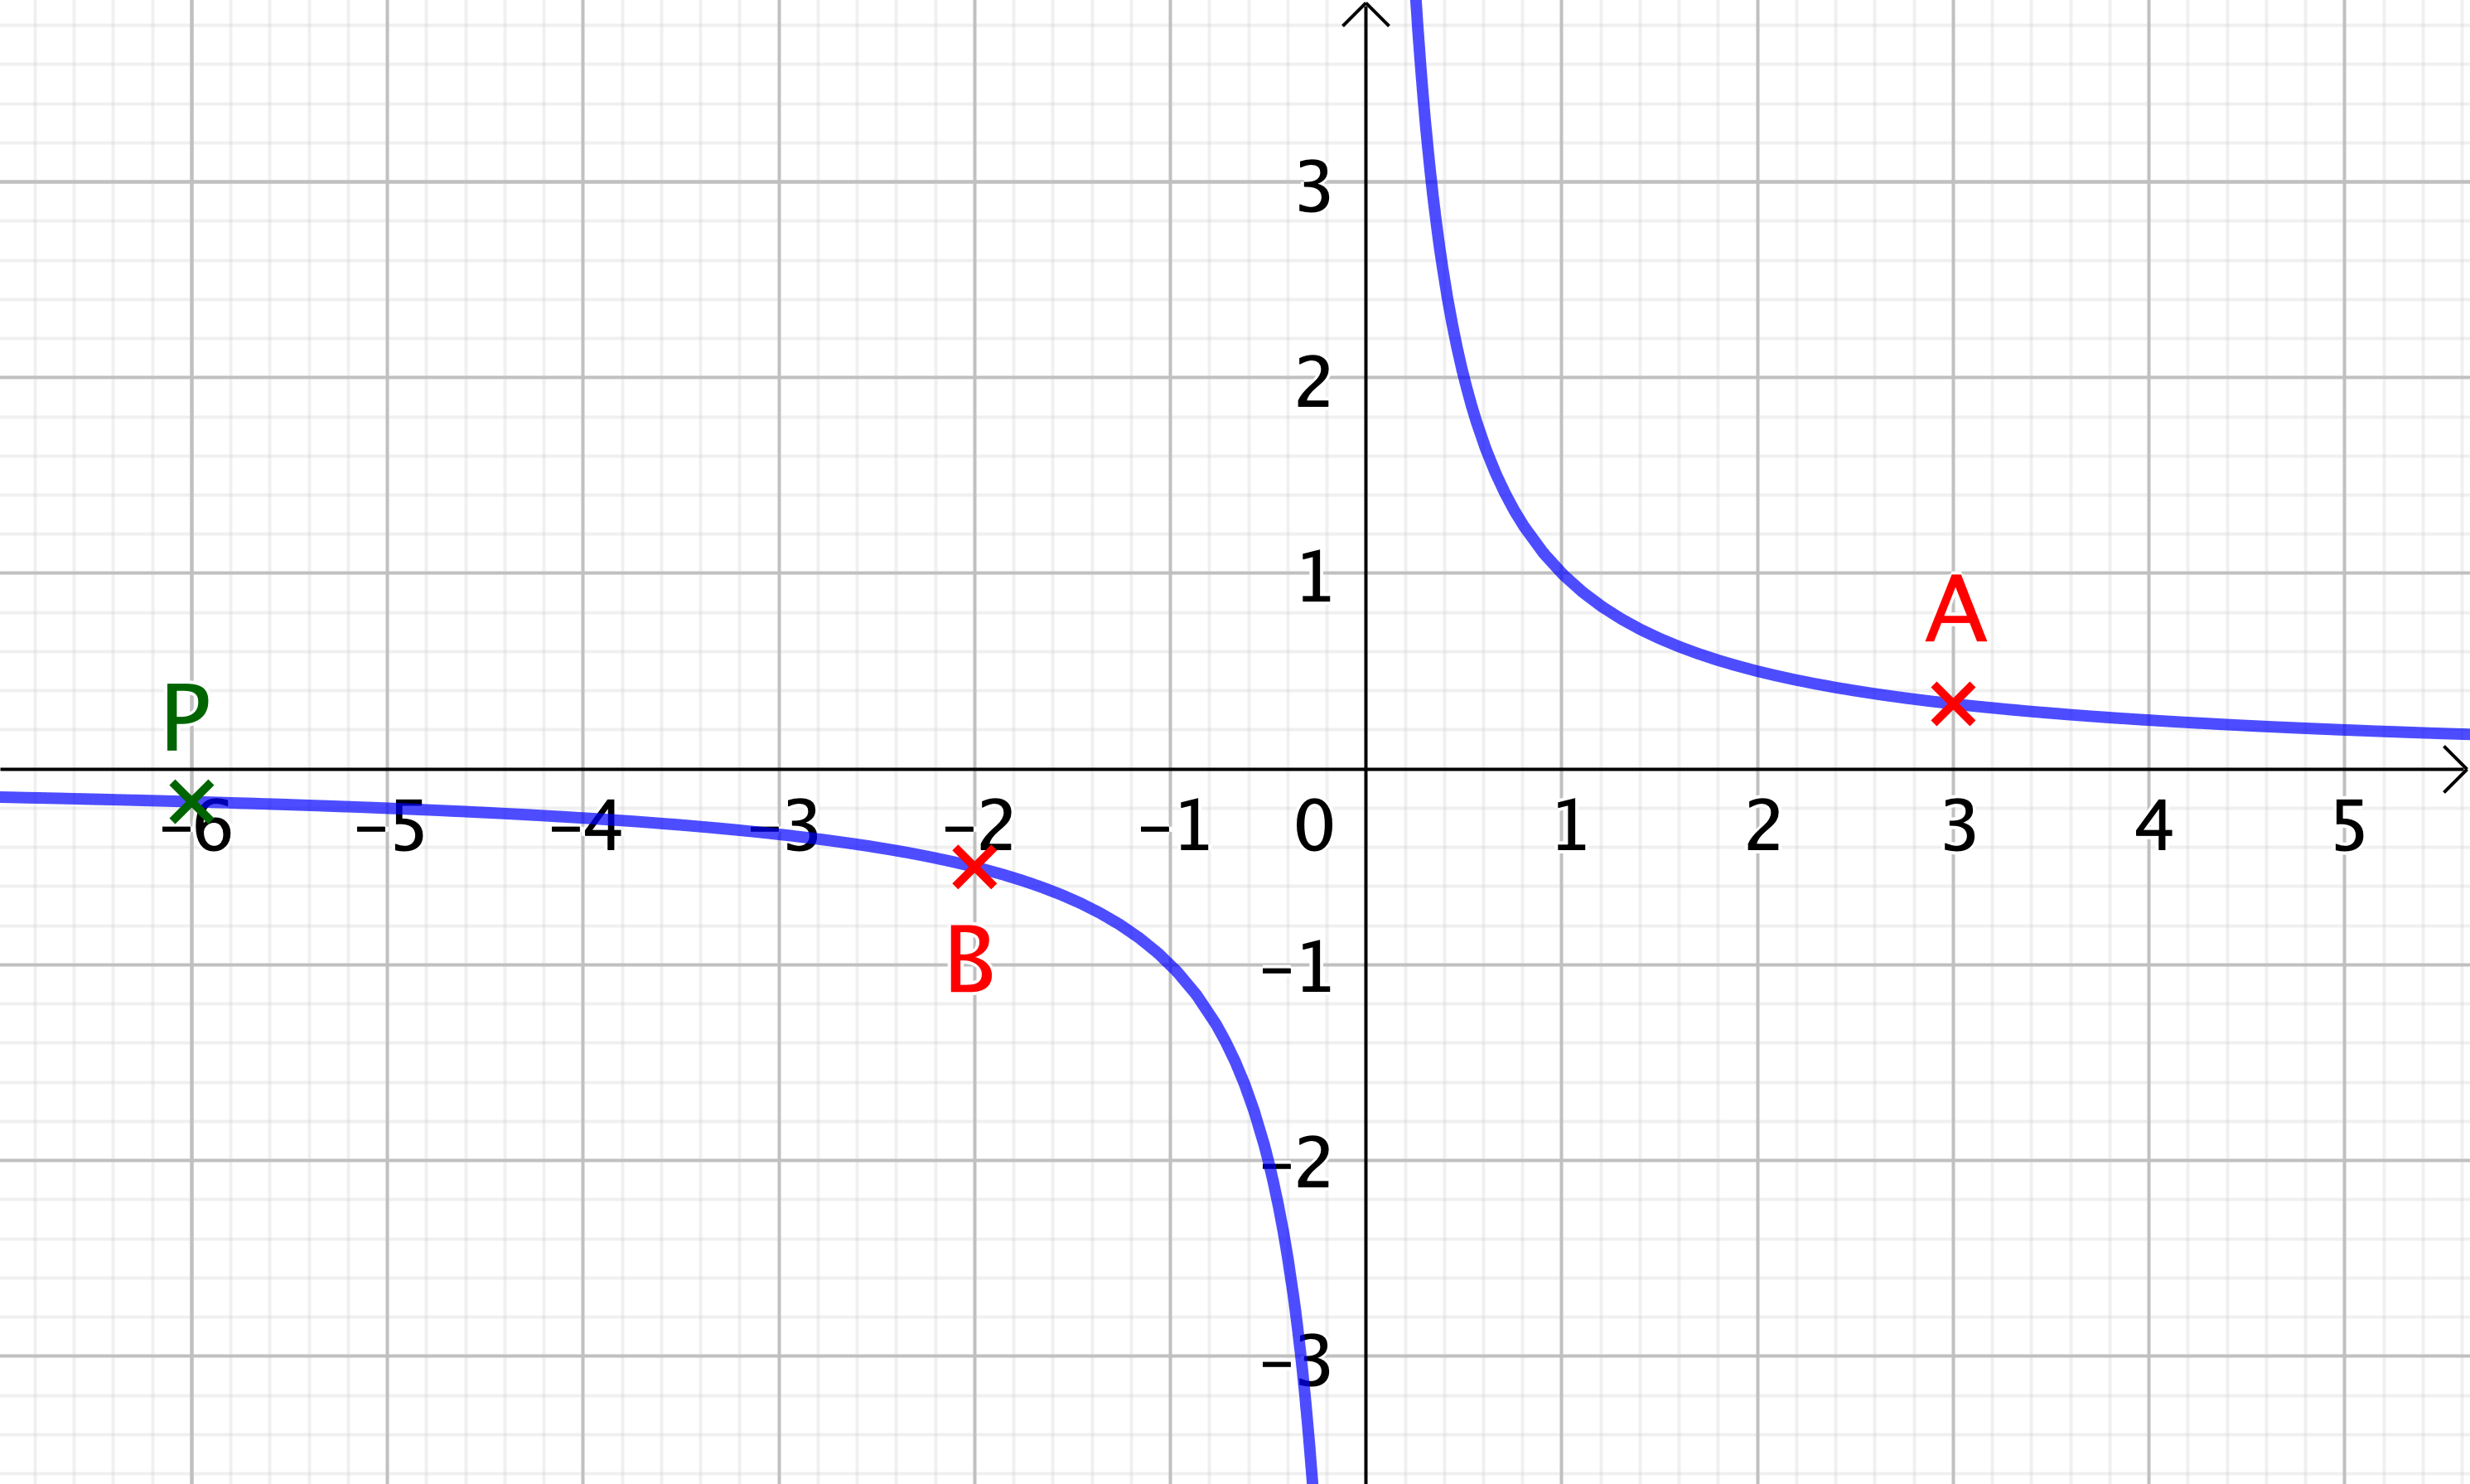
\includegraphics[scale = .8]{addition-on-parabolas/conjecture/a-and-b-diff-signs.png}}
	
	\smallskip
	Cas où $a < 0$ et $b > 0$
\end{multicols}
	
\begin{center}
	\footnotesize
	\itshape

	\fbox{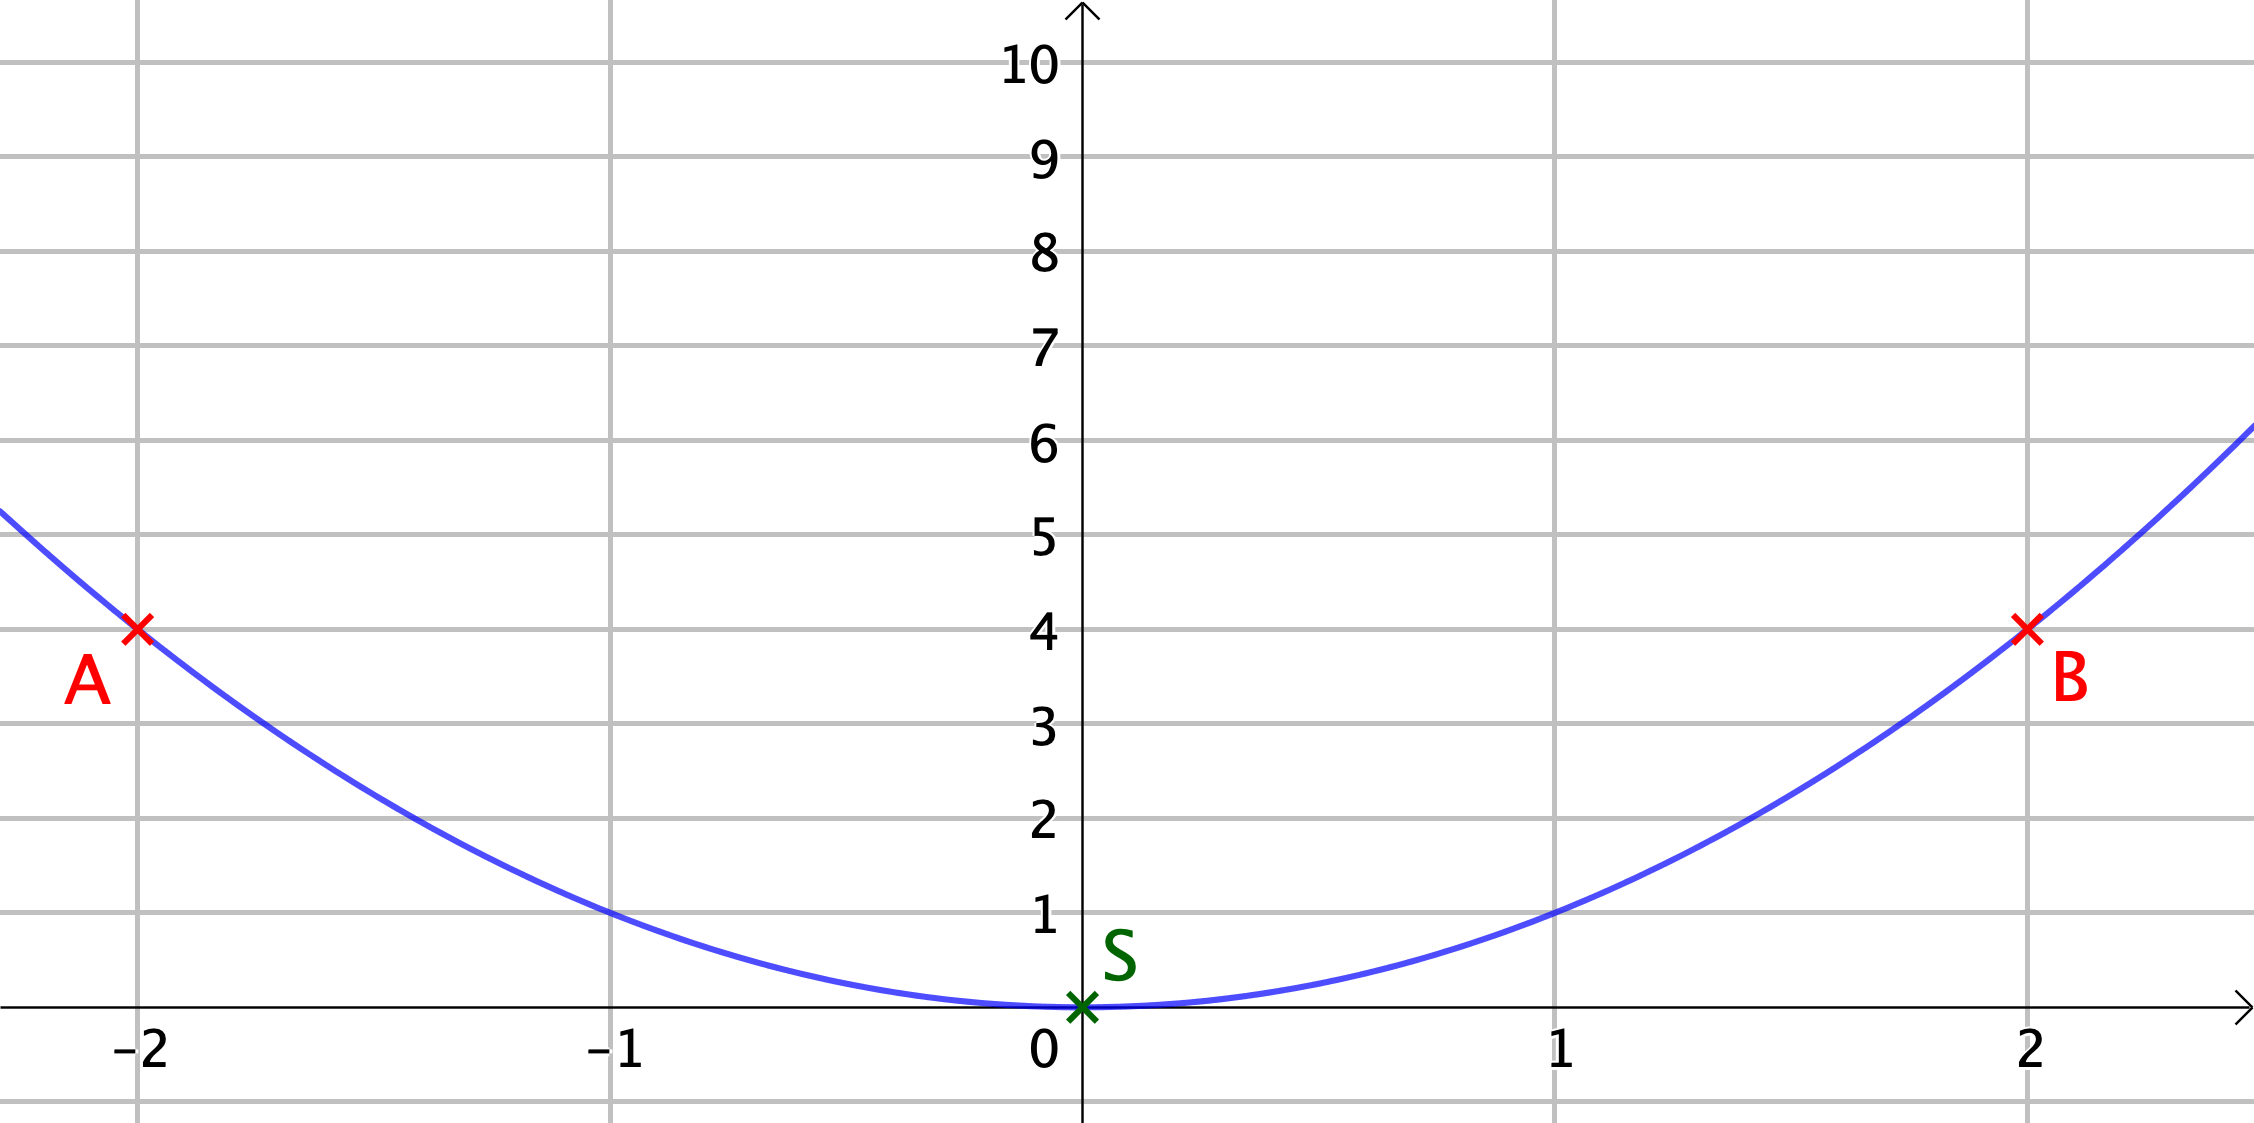
\includegraphics[scale = .8]{addition-on-parabolas/conjecture/a-and-b-opposite.png}}
	
	\smallskip
	Cas où $a = -b$
\end{center}


\newpage

Pour mieux voir ce qu'il se passe, traçons quelques droites. Voici ce que cela donne.

\begin{multicols}{2}
	\center
	\footnotesize
	\itshape

	\fbox{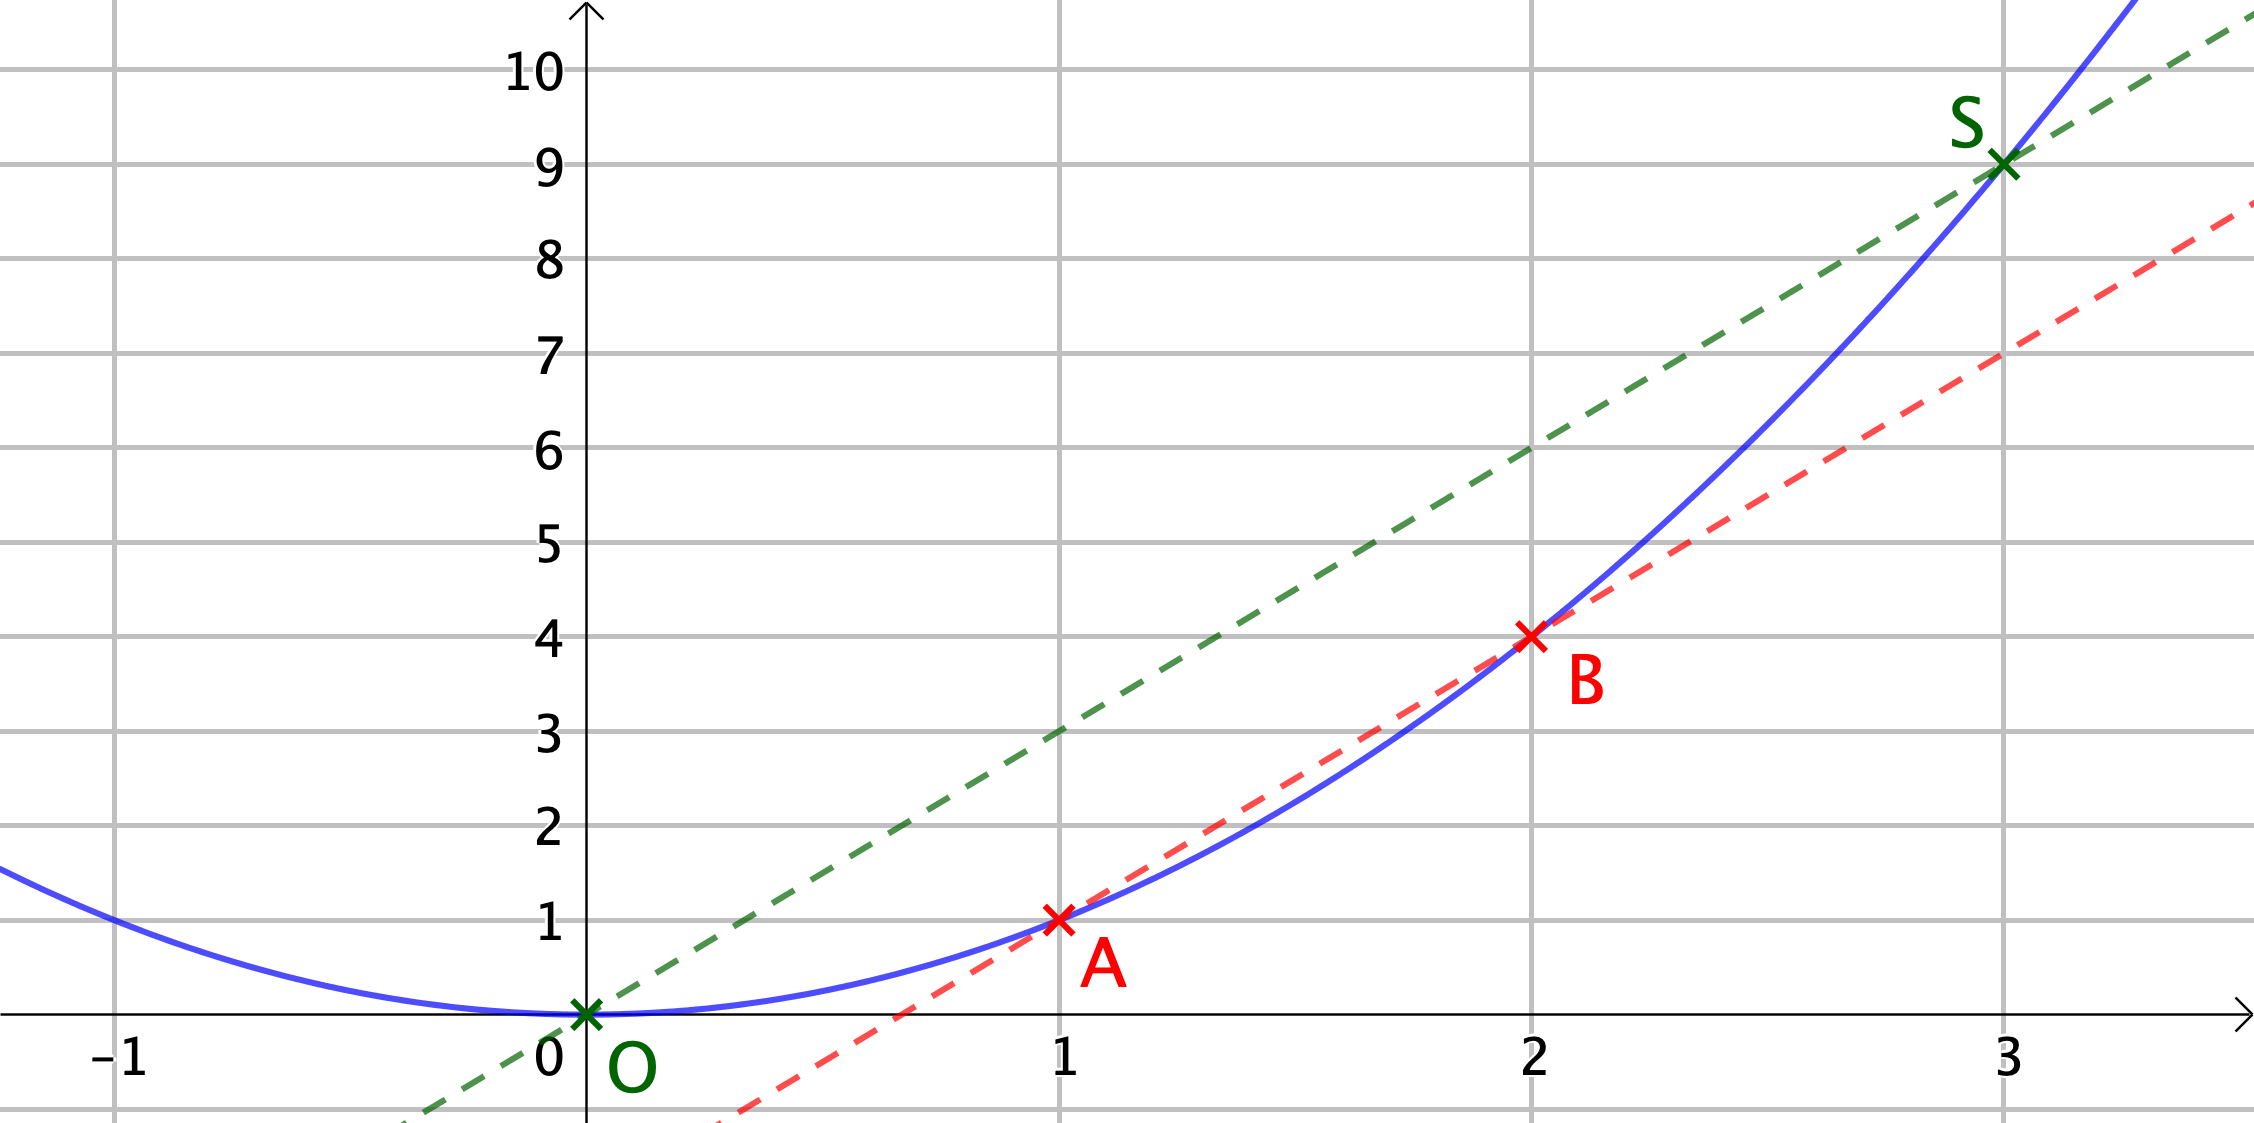
\includegraphics[scale = .8]{addition-on-parabolas/conjecture/a-and-b-positive-with-lines.png}}
	
	\smallskip
	Cas où $a > 0$ et $b > 0$

	\columnbreak
	
	\fbox{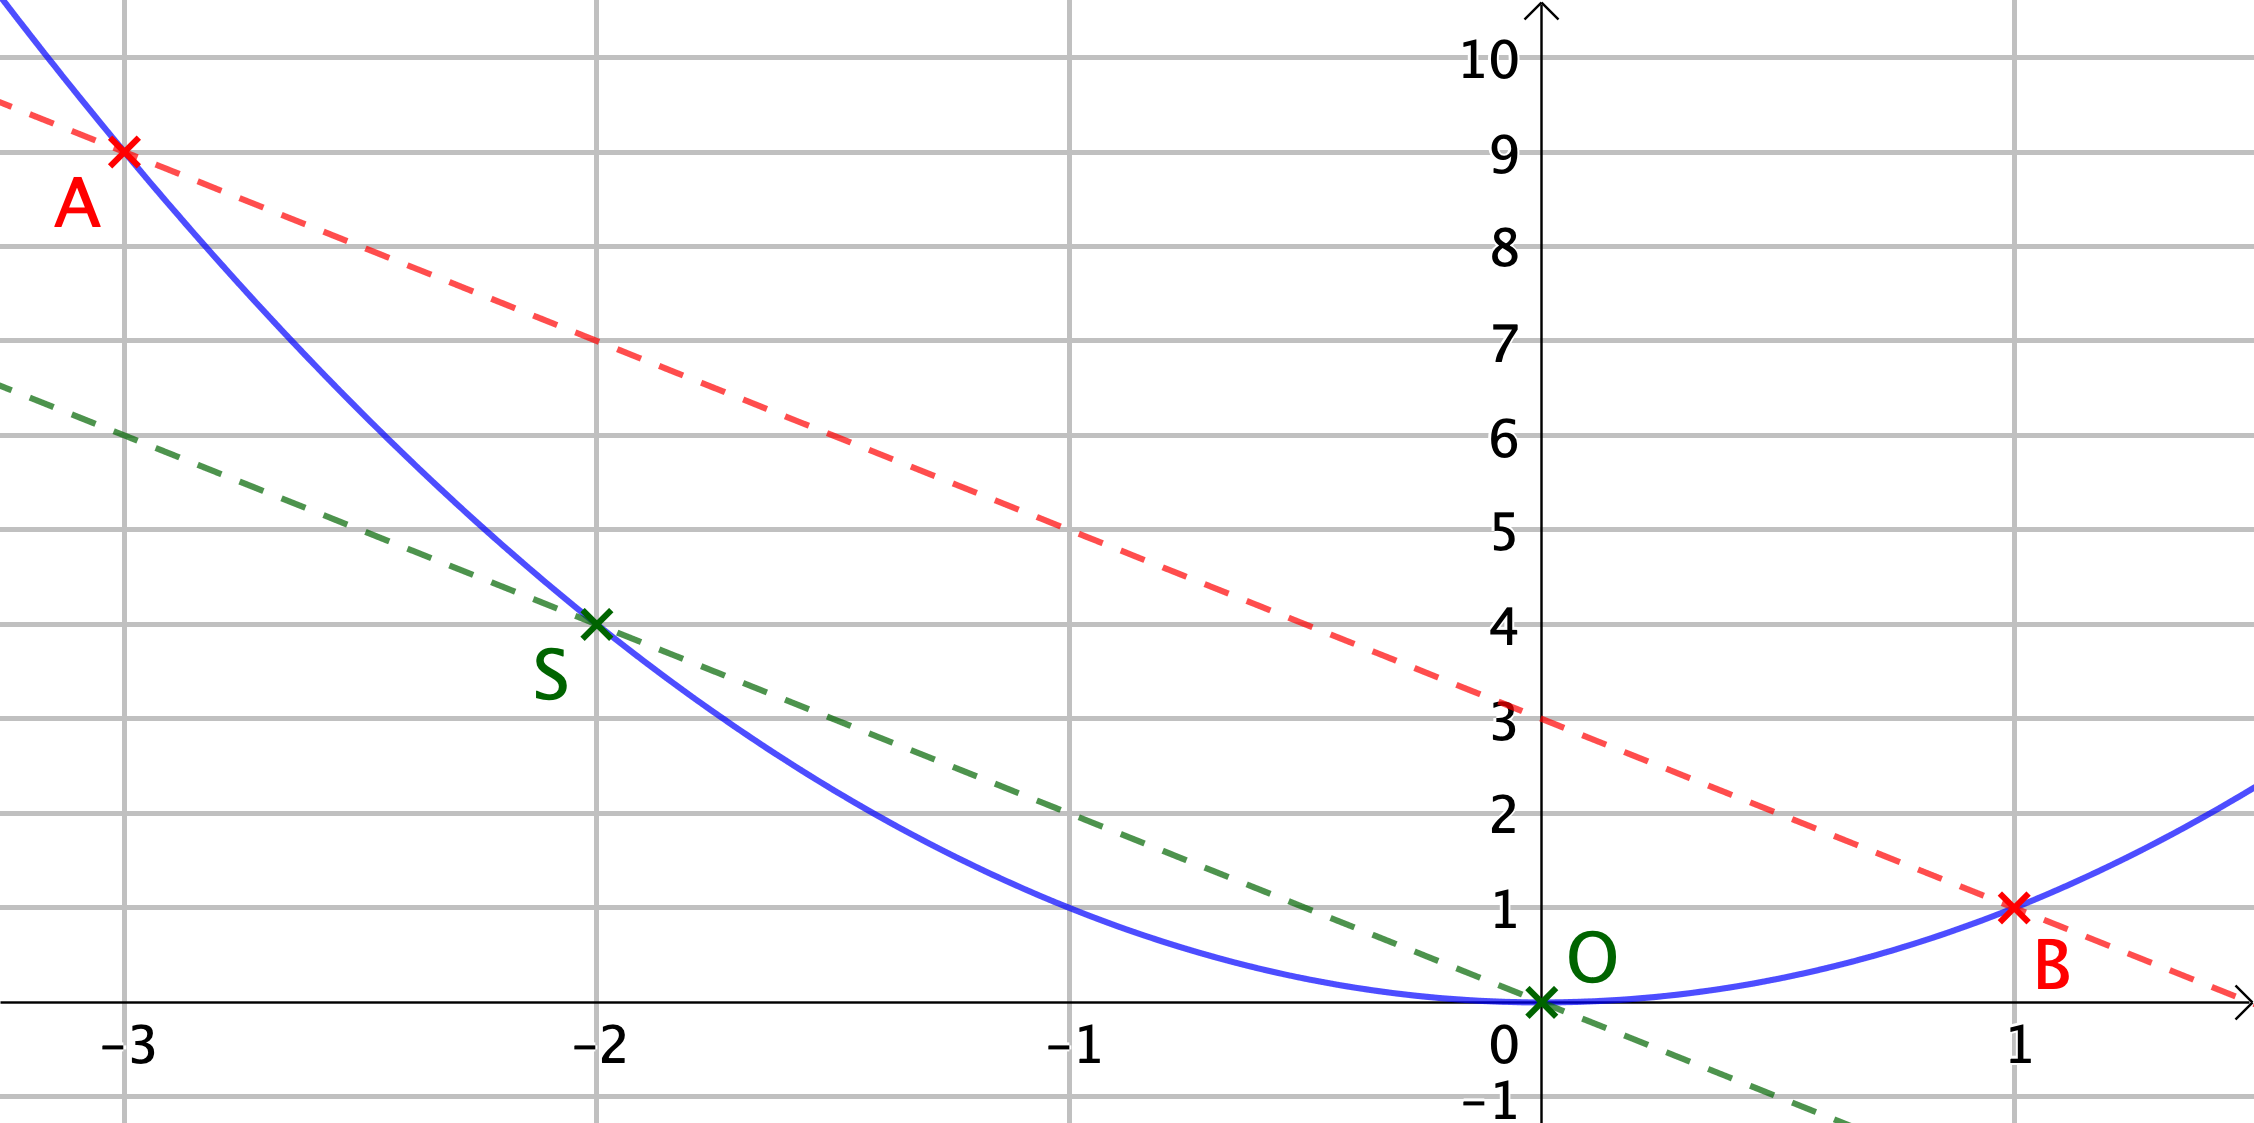
\includegraphics[scale = .8]{addition-on-parabolas/conjecture/a-and-b-diff-signs-with-lines.png}}
	
	\smallskip
	Cas où $a < 0$ et $b > 0$
\end{multicols}
	
\begin{center}
	\footnotesize
	\itshape

	\fbox{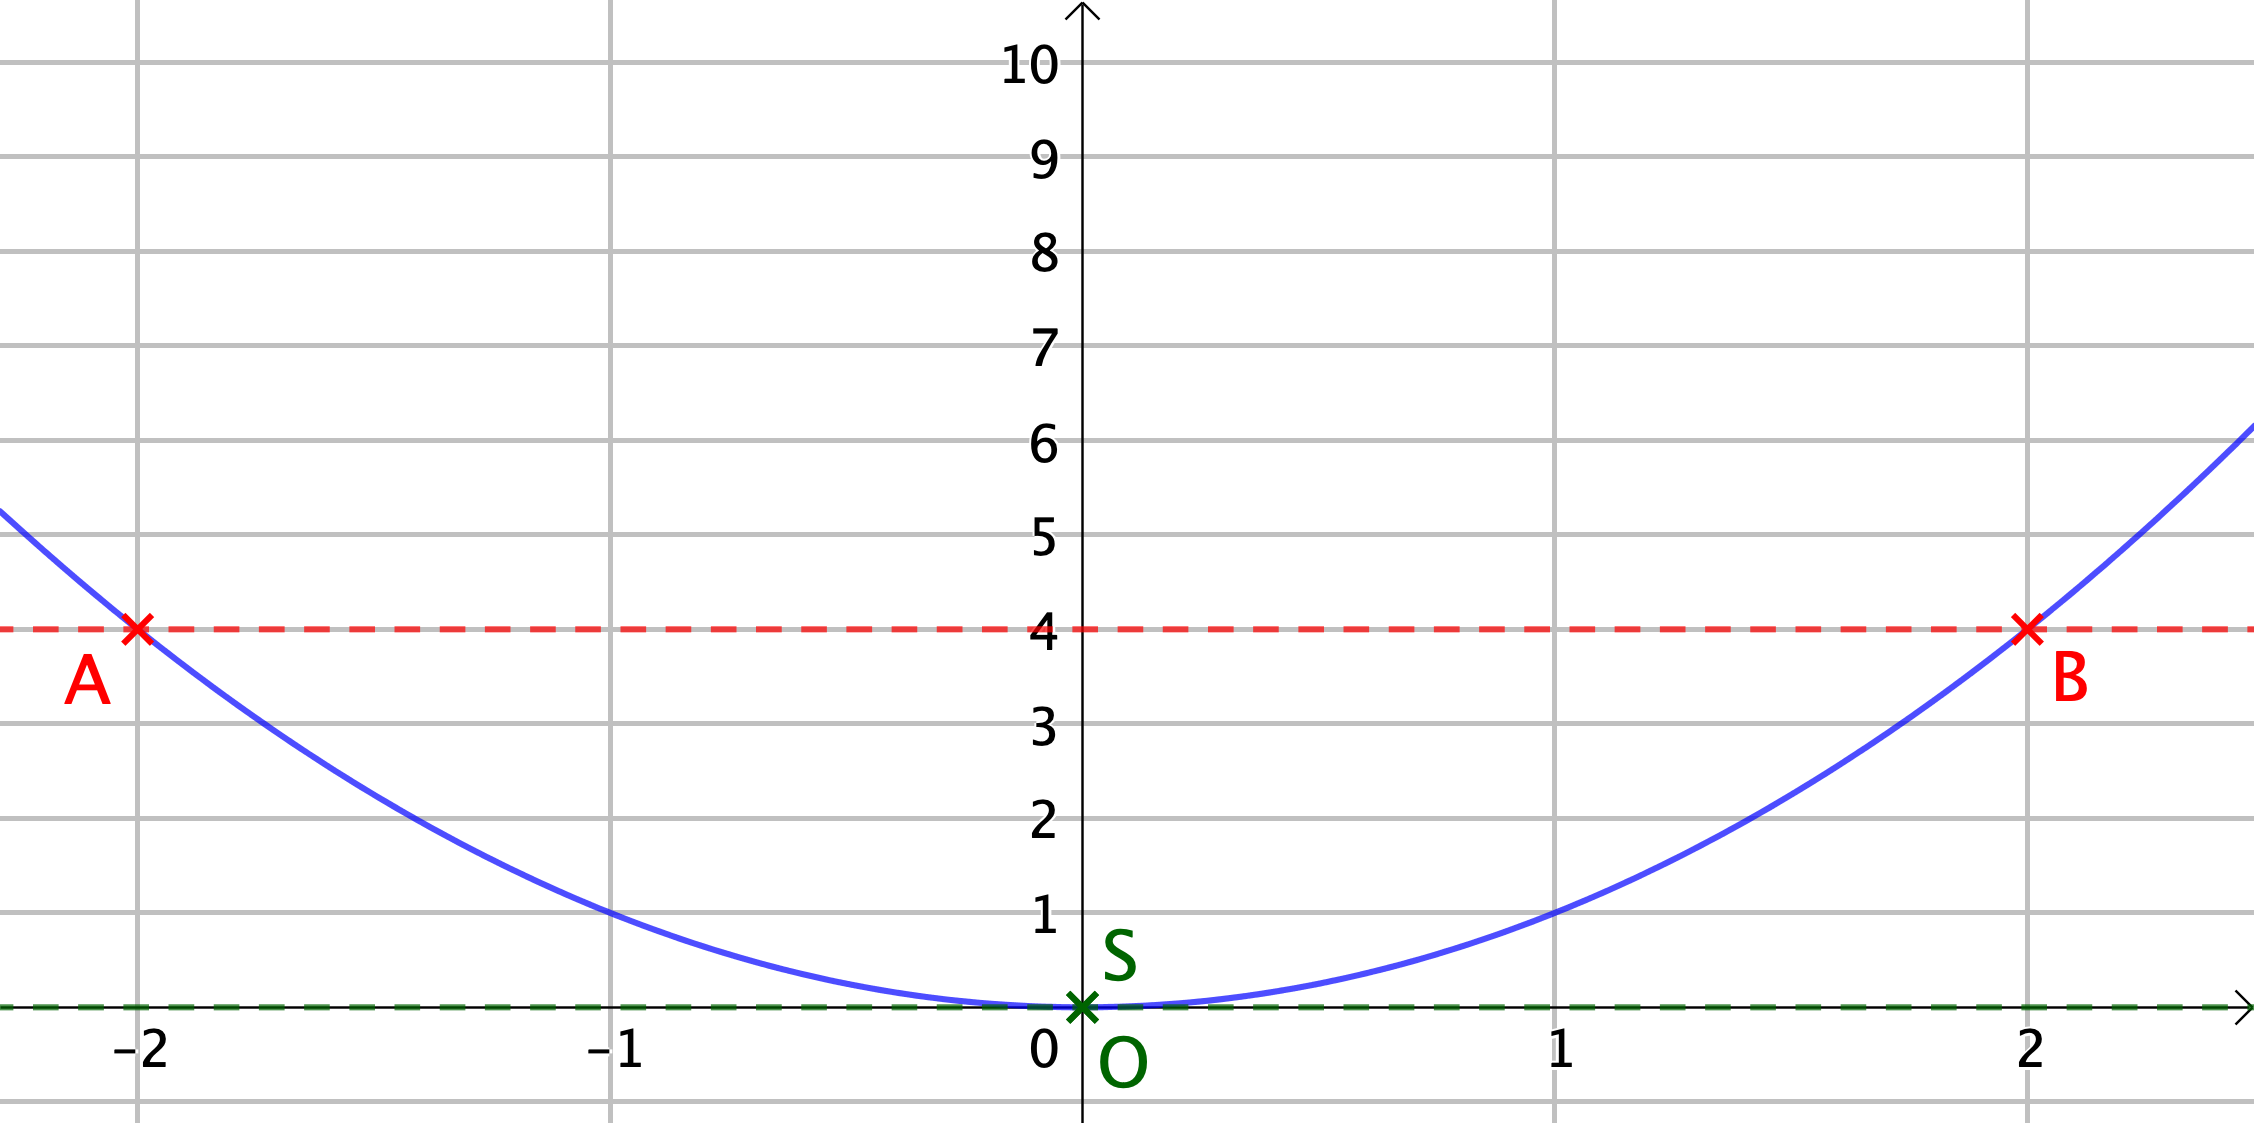
\includegraphics[scale = .8]{addition-on-parabolas/conjecture/a-and-b-opposite-with-lines.png}}
	
	\smallskip
	Cas où $a = -b$
\end{center}


\medskip

Il devient évident de conjecturer que le point $S$ se construit géométriquement comme suit.

\begin{enumerate}
	\item \label{point-1} Si $x_A \neq \pm \, x_B$ alors on construit la parallèle à $(AB)$ passant par $O$ l'origine du repère. Le point $S$ est le second point d'intersection de cette parallèle avec $\setgeo{P}$  \emph{(notons qu'une droite coupe $\setgeo{P}$ en au plus deux points)}.

	\item Si $x_A = - x_B$ alors $S = O$ . Notons au passage que l'on peut voir ceci comme un cas limite du précédent avec un point d'intersection \squote{double}.

	\item Si $x_A = x_B \neq 0$ , on procède comme au point (\ref{point-1}) mais avec la parallèle à la tangente en $A$ à la parabole $\setgeo{P}$ .
\end{enumerate}


La section qui suit va valider cette conjecture qui donne un moyen très capillotracté de calculer une somme de deux réels via la parabole $\setgeo{P}$ .
Plus sérieusement, la construction ci-dessus est une propriété géométrique très jolie de la parabole $\setgeo{P}$ .



\section{Comprendre partiellement\dots}

Essayons de voir, sans chercher à être trop rigoureux, la raison de ce phénomène au travers de deux situations instructives. Ci-après $\setgeo{D}_k \, /\!/ \, \setgeo{d}_k$ pour $k \in \{ 1 \,; 2\}$ et $F$ est le point d'intersection des deux demi-droites.


\medskip


Dans la 1\iere{} situation représentée ci-dessous, nous avons un rayon initial "allant vers $F$" et faisant avec la direction de la demi-droite $\setgeo*{d}{2}$ un angle géométrique $\alpha \in \intervalO{0}{\frac{\pi}{2}}$ , puis au bout de deux rebonds, nous obtenons un rayon "allant vers $F$" avec un angle géométrique de mesure $\alpha + 2\theta$ relativement à la direction de $\setgeo*{d}{2}$.


\medskip


\begin{center}
	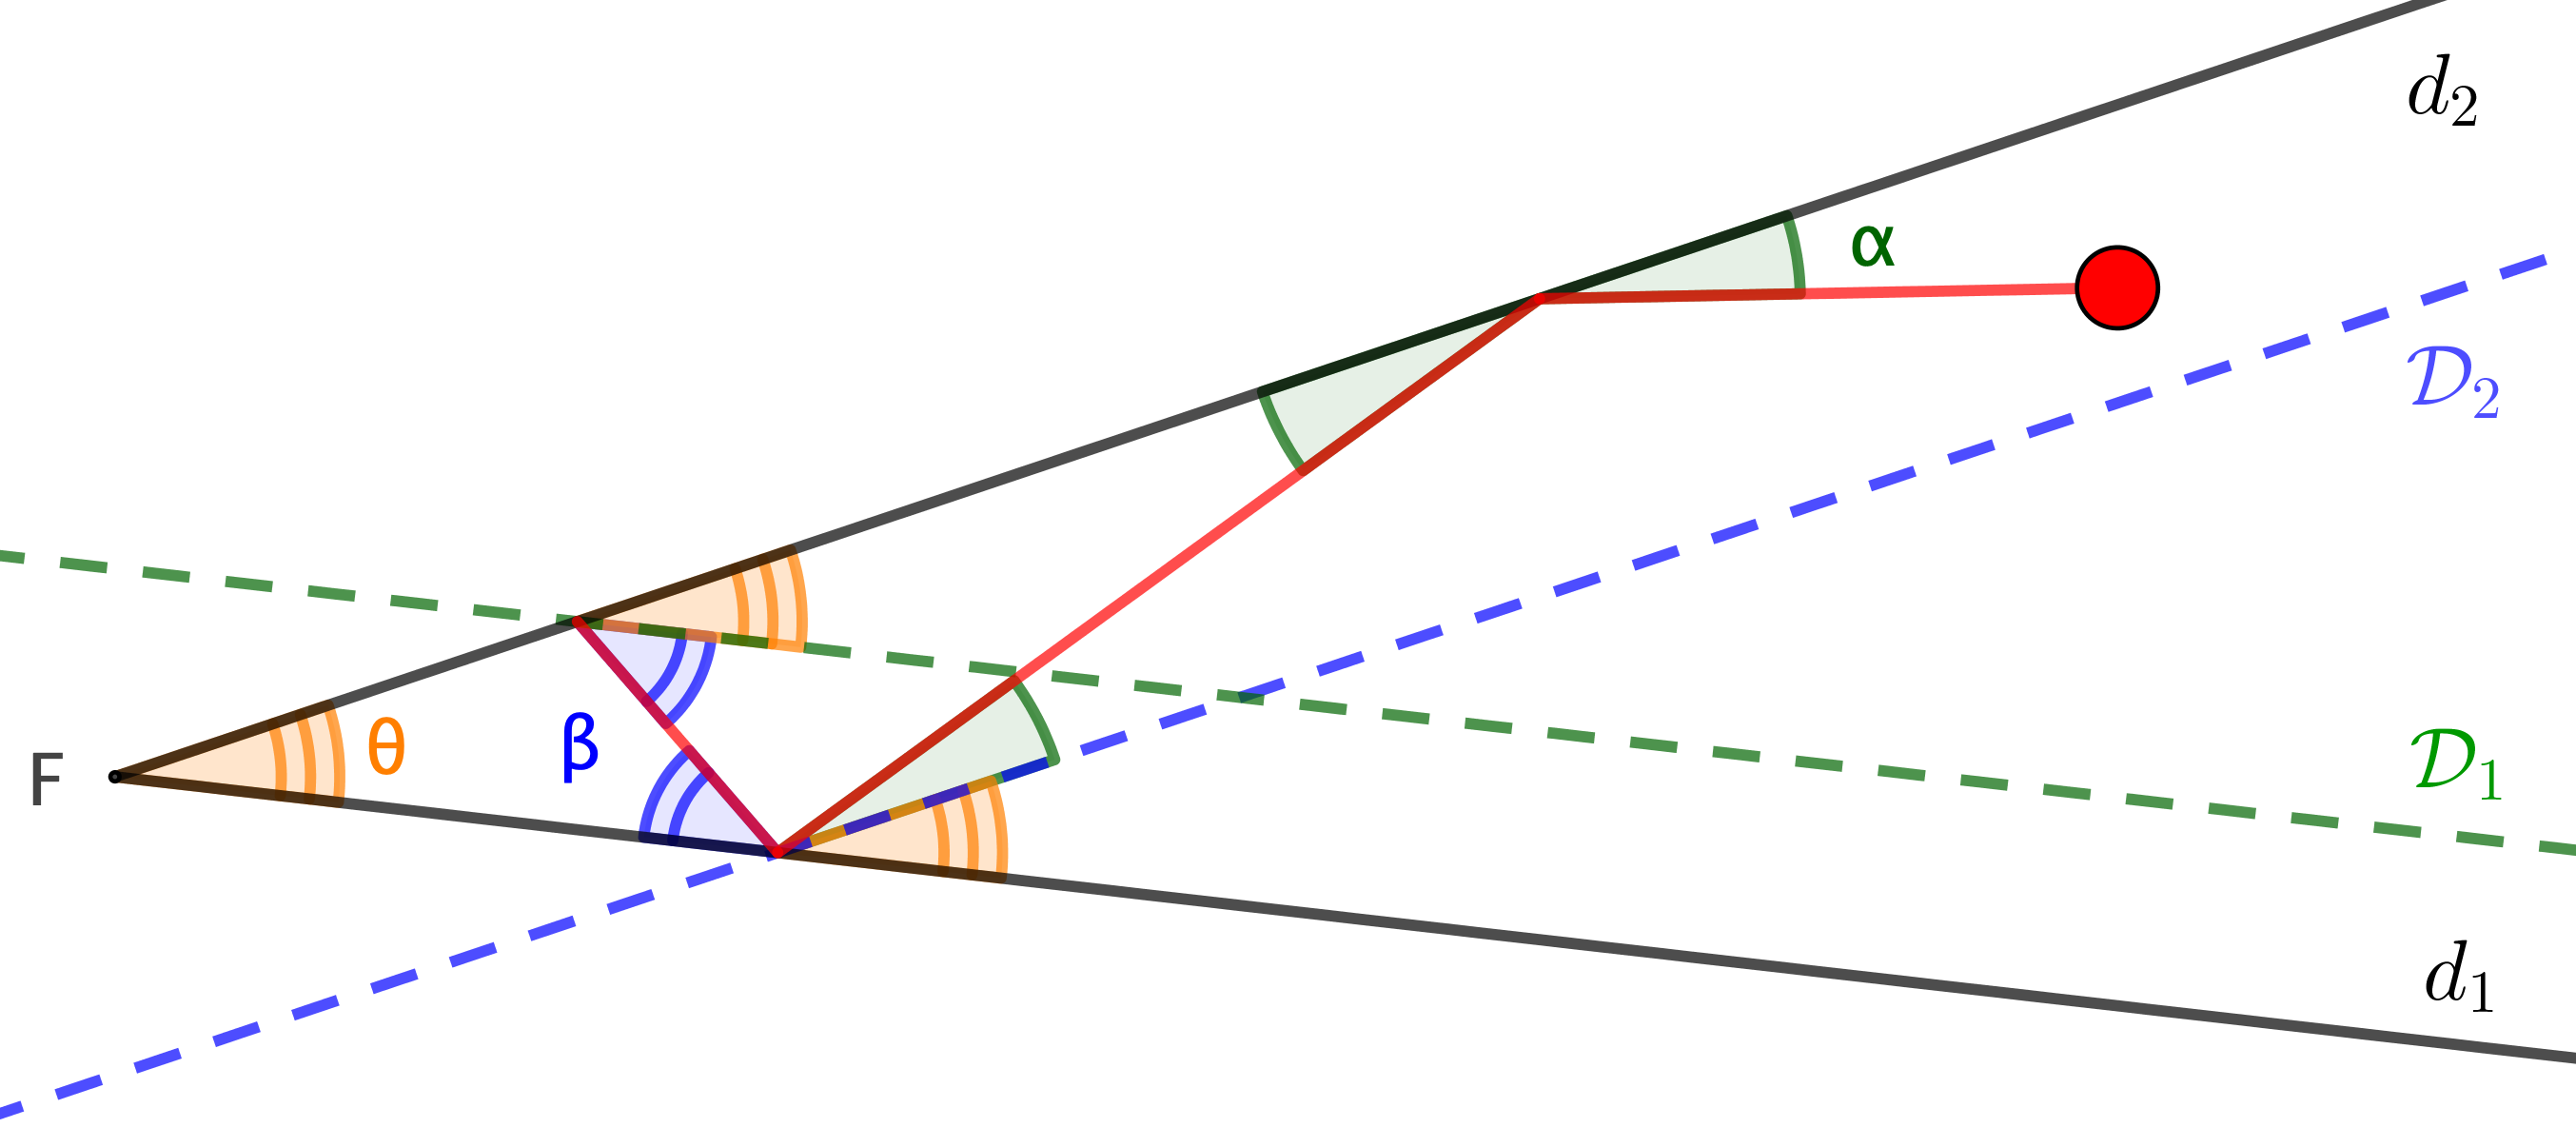
\includegraphics[width=12cm]{basic-math-pool/analysis-1.png}
	
	\itshape\small
	Situation n\textdegree1
	\label{situtation-1}
\end{center}


\medskip


Dans la 2\ieme{} situation ci-après, nous avons un rayon initial "allant à l'opposé de $F$" et faisant  avec la direction de $\setgeo*{d}{2}$ un angle géométrique $\alpha \in \intervalO{0}{\frac{\pi}{2}}$ , puis au bout de deux rebonds, nous obtenons un rayon "allant à l'opposé de $F$" avec un angle géométrique mesurant $\alpha - 2\theta$ relativement à la direction de $\setgeo*{d}{2}$.


\medskip


\begin{center}
	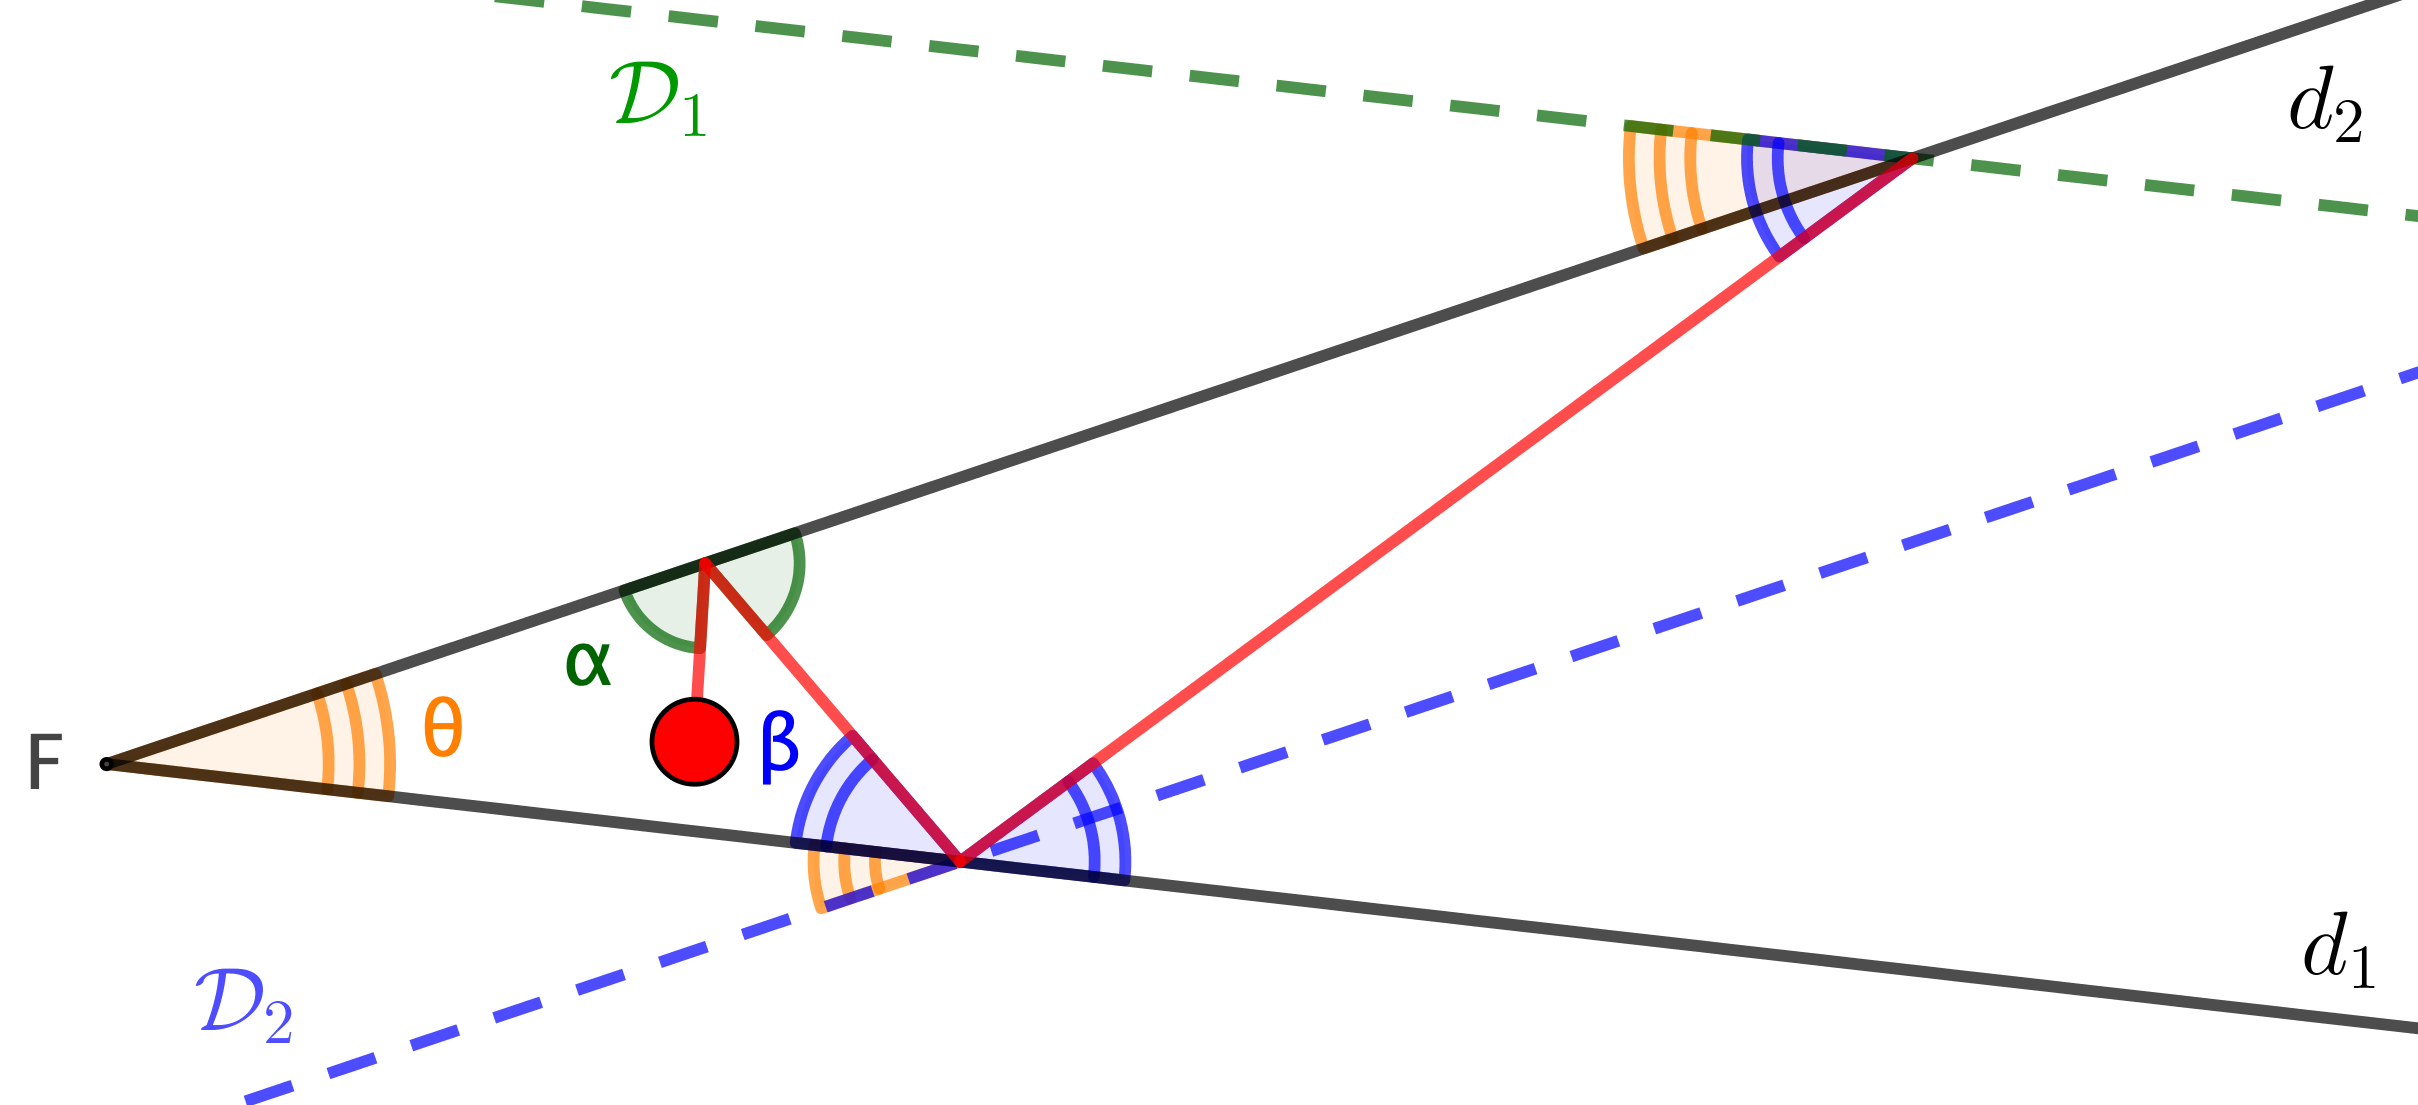
\includegraphics[width=12cm]{basic-math-pool/analysis-2.png}
	
	\itshape\small
	Situation n\textdegree2
	\label{situtation-2}
\end{center}


\medskip

Imaginons que notre bille soit d'abord confrontée à la situation n\textdegree1. Au bout de deux rebonds, l'angle relativement à $\setgeo*{d}{2}$ passe de $\alpha_0 = \alpha$ à $\alpha_1 = \alpha + 2 \theta$. Une suite successive de situations n\textdegree1 va donc faire augmenter l'angle par rapport à la direction de $\setgeo*{d}{2}$. Il arrivera donc un moment où la situation n\textdegree2 arrivera, excepté si l'on obtient un rebond perpendiculaire à $\setgeo*{d}{2}$. Nous ignorons ici ce cas qui sera géré dans notre démonstration.

Une fois que la situation n\textdegree2 se présente, nous avons des angles de plus en plus petit relativement à $\setgeo*{d}{2}$ jusqu'à arriver au dernier rebond possible après lequel la bille s'éloignera indéfiniment. Voilà une explication partielle du phénomène.


\section{Notations pour la suite}

Tous les angles sont orientés et confondus abusivement avec leur mesure principale.
\begin{enumerate}
	\item $\setgeo*{d}{1}$ et $\setgeo*{d}{2}$ sont deux demi-droites d'origine $F$ et telles que $\theta = \langle \setgeo*{d}{1} \,; \setgeo*{d}{2} \rangle \in \intervalO{0}{\dfrac{\pi}{2}}$ .

	\item $S$, le point de départ, est tel que $S \notin \setgeo*{d}{1} \cup \setgeo*{d}{2}$ et $\tau = \langle \setgeo*{d}{1} \,; [FS) \rangle \in \intervalO{0}{\theta}$ .
	
	\item Pour tout point $M$ du plan, nous noterons $H_M$ sont projeté orthogonal sur $\setgeo*{d}{2}$.
	
	\item Pour tout point $M$ qui est sur le trajet de la bille, mais pas sur $\setgeo*{d}{2}$, si $D_M$ est un point tel que $\vect{MD_M}$ indique la direction et le sens du trajet "sortant" de $M$, nous notons $\sigma_M = \langle \vect{MH_M} \,; \vect{MD_M} \rangle$.
\end{enumerate}


\medskip


\begin{center}
	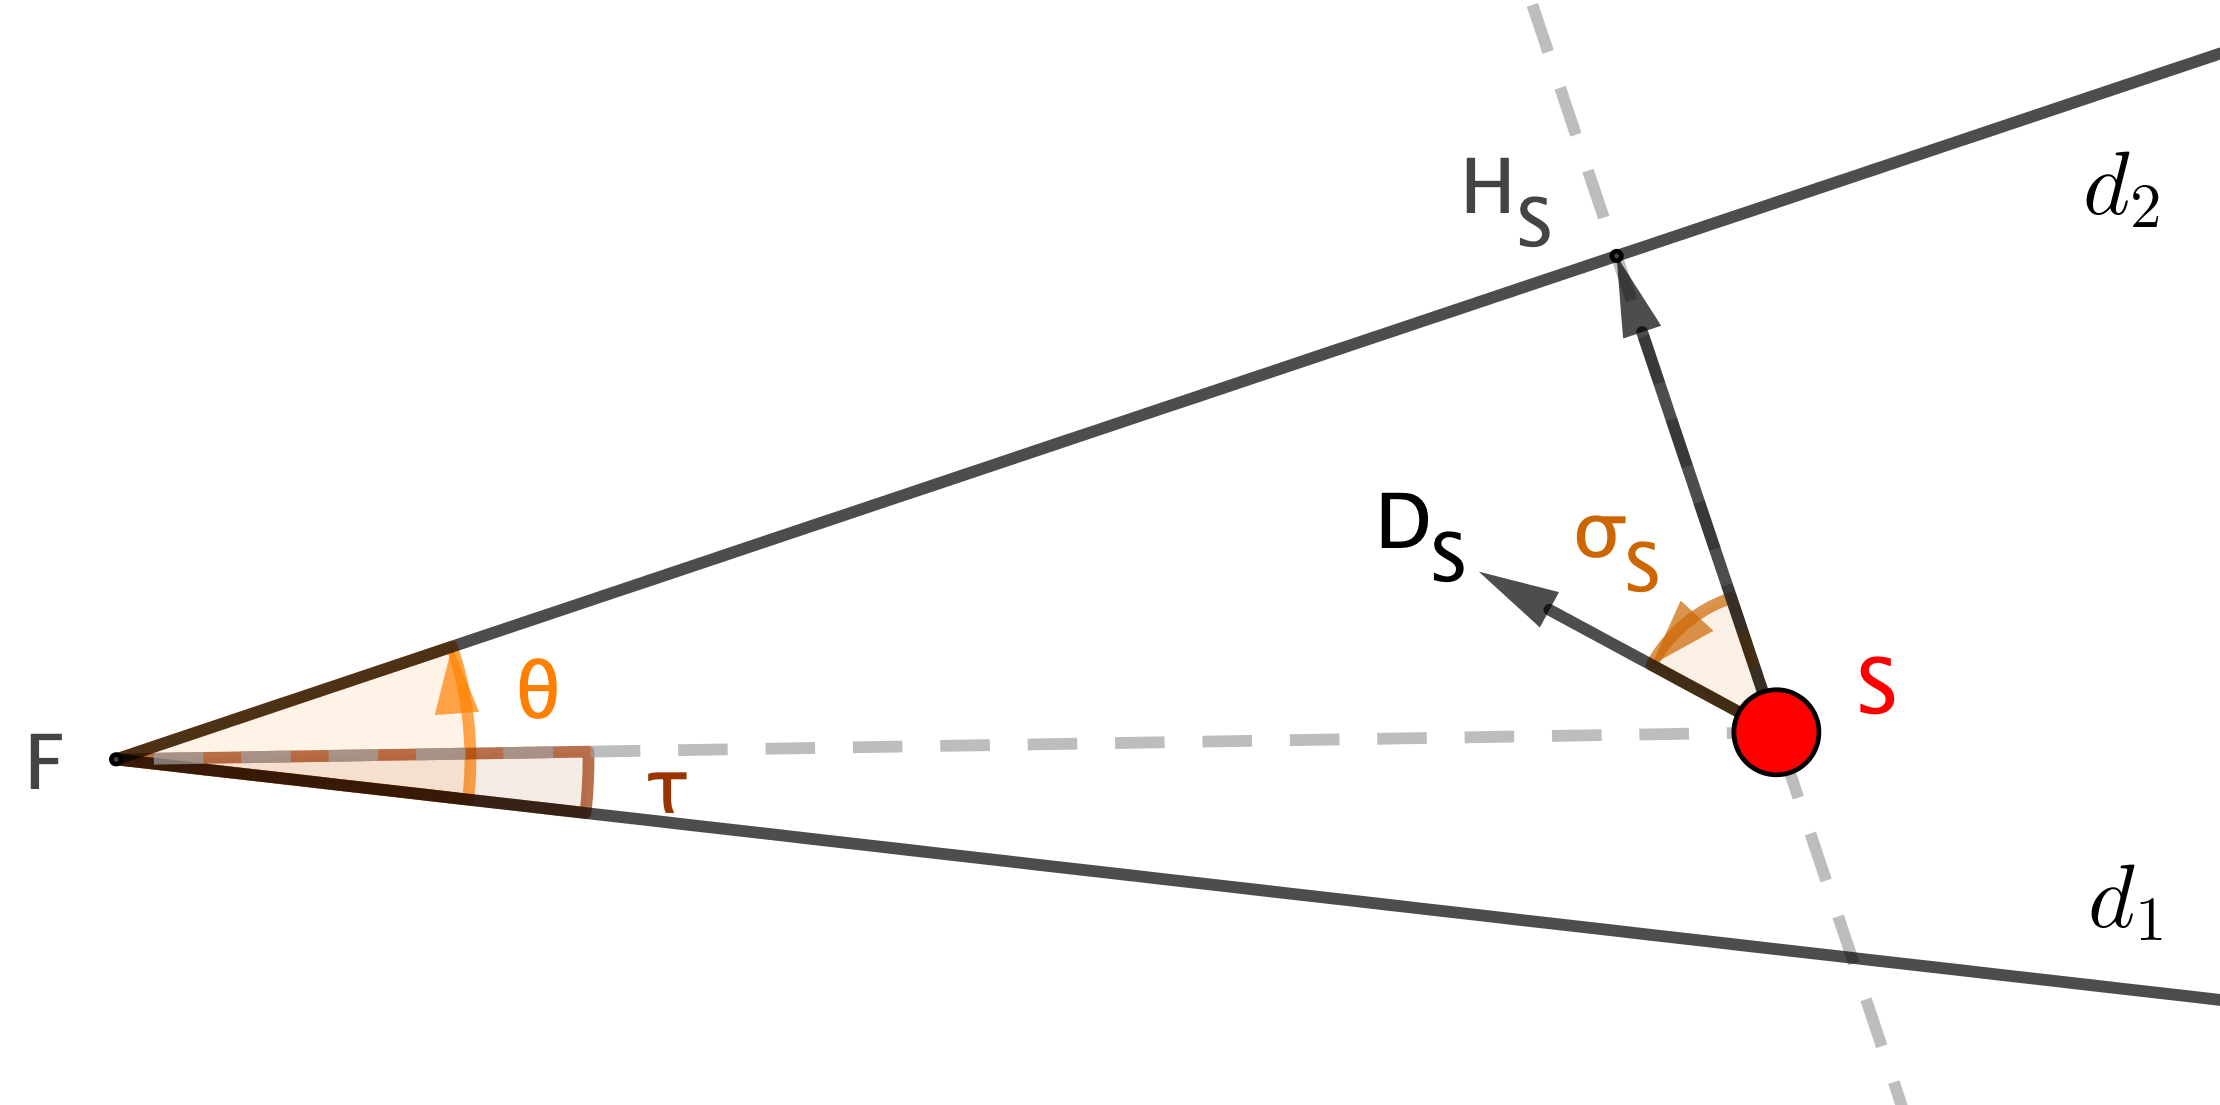
\includegraphics[width=12cm]{content/proof-notations.png}
	
	\itshape\small
	Notations pour la suite
\end{center}





\section{Où se fait le 1\ier{} rebond ?}
\label{1st-bounce}

\begin{fact}
	Nous avons les cas initiaux suivants.
	
	\begin{itemize}[label = \small\textbullet]
		\item Il n'y a aucun rebond si et seulement si $\sigma_S \in \intervalC{- \dfrac{\pi}{2} - \theta}{- \dfrac{\pi}{2}}$.
		
		\item La bille va directement vers $F$ si et seulement si $\sigma_S = \dfrac{\pi}{2} - \theta + \tau$.

		\item Le 1\ier{} rebond se fait sur $\setgeo*{d}{1}$ si et seulement si $\sigma_S \in \intervalOC{\dfrac{\pi}{2} - \theta + \tau}{\pi} \cup \intervalO{- \pi}{- \dfrac{\pi}{2} - \theta}$.

		\item Le 1\ier{} rebond se fait sur $\setgeo*{d}{2}$ si et seulement si $\sigma_S \in \intervalO{- \dfrac{\pi}{2}}{\dfrac{\pi}{2} - \theta + \tau}$.
	\end{itemize}

\end{fact}

\begin{proof}
	Tout est contenu dans les deux dessins suivants où $\setgeo*{D}{k} \, /\!/ \, \setgeo*{d}{k}$ pour $k \in \{ 1 \,; 2\}$.

	\medskip

	\begin{center}
		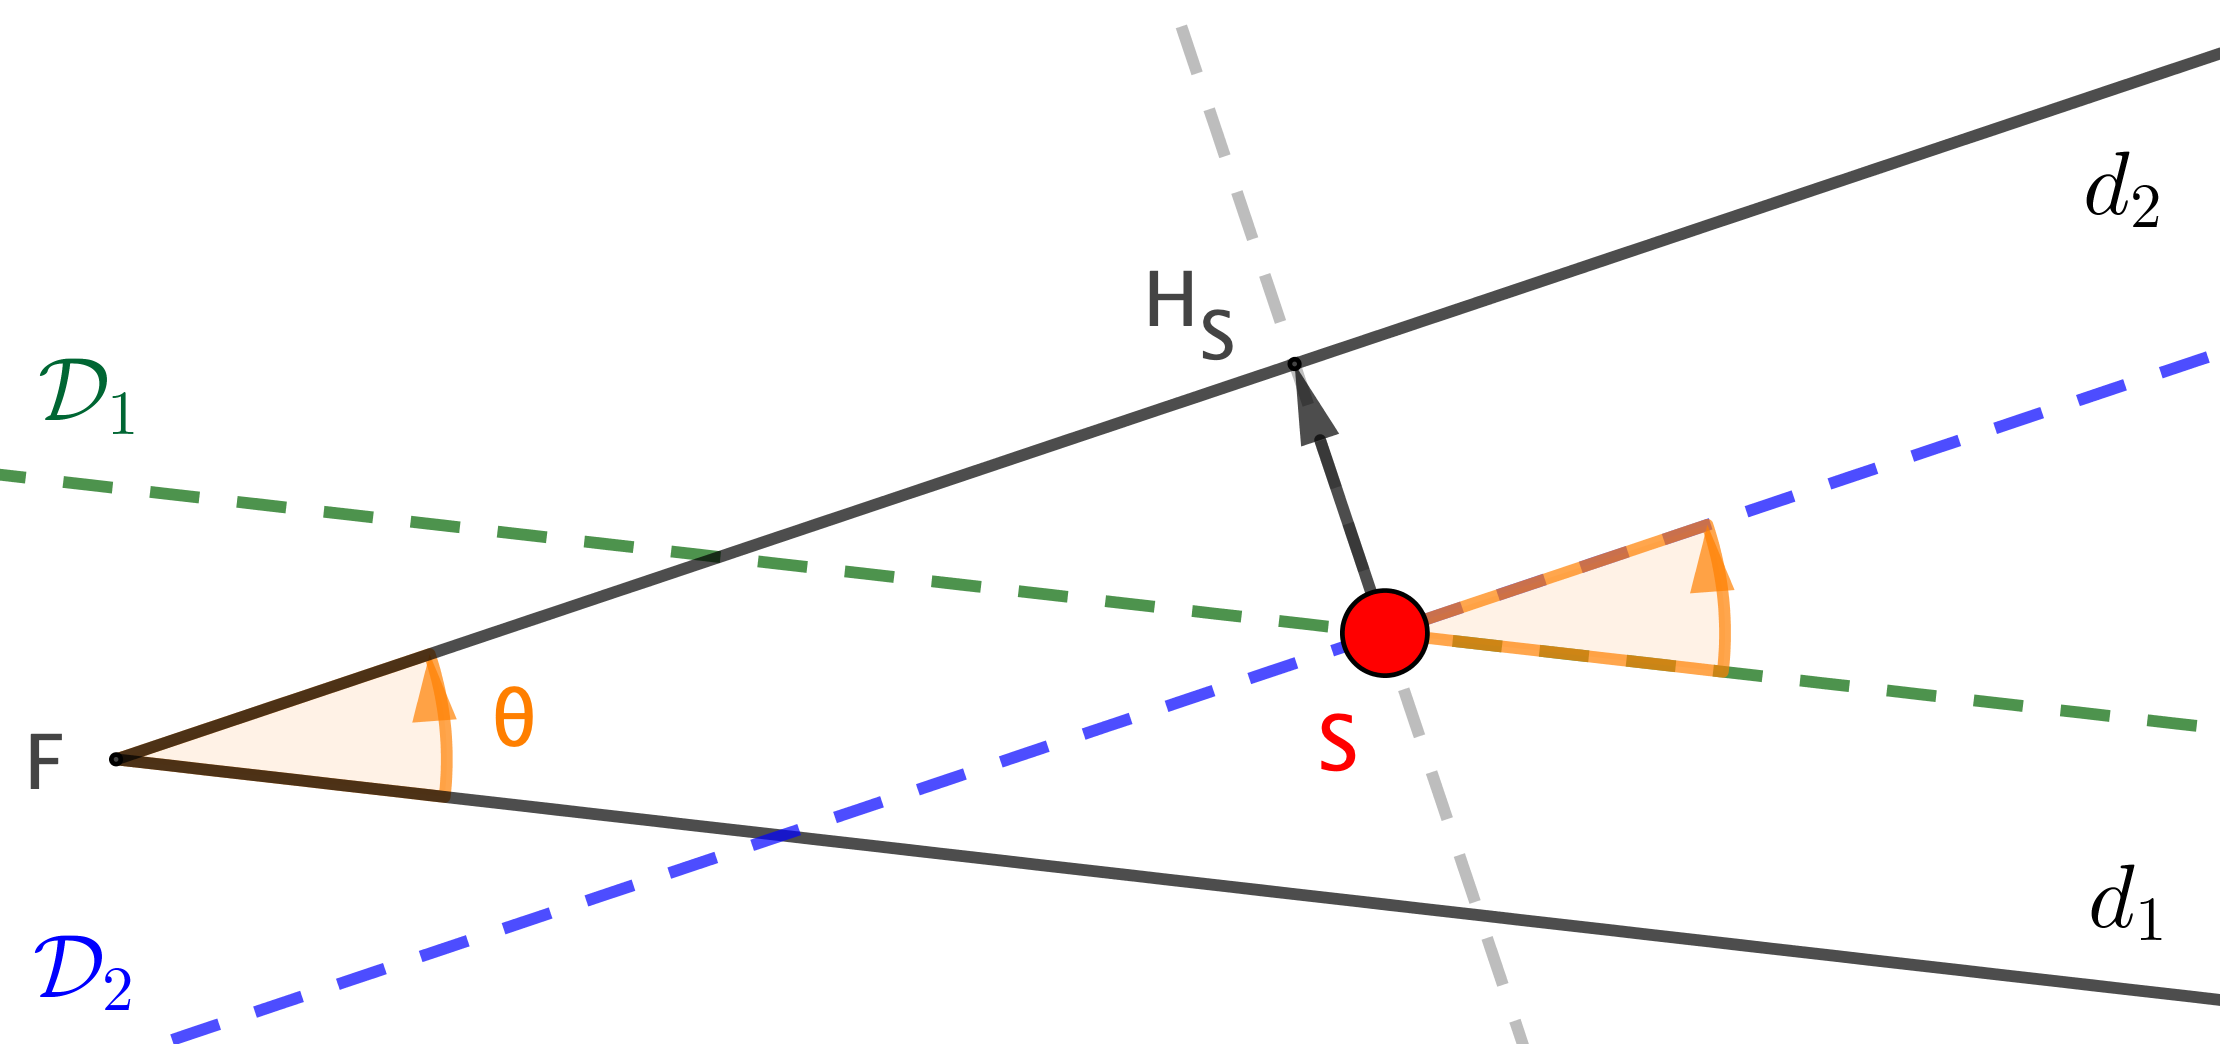
\includegraphics[width=12cm]{content/proof-no-bounce.png}

		\itshape\small
		Aucun 1\ier{} rebond
	\end{center}

	\medskip

	\begin{center}
		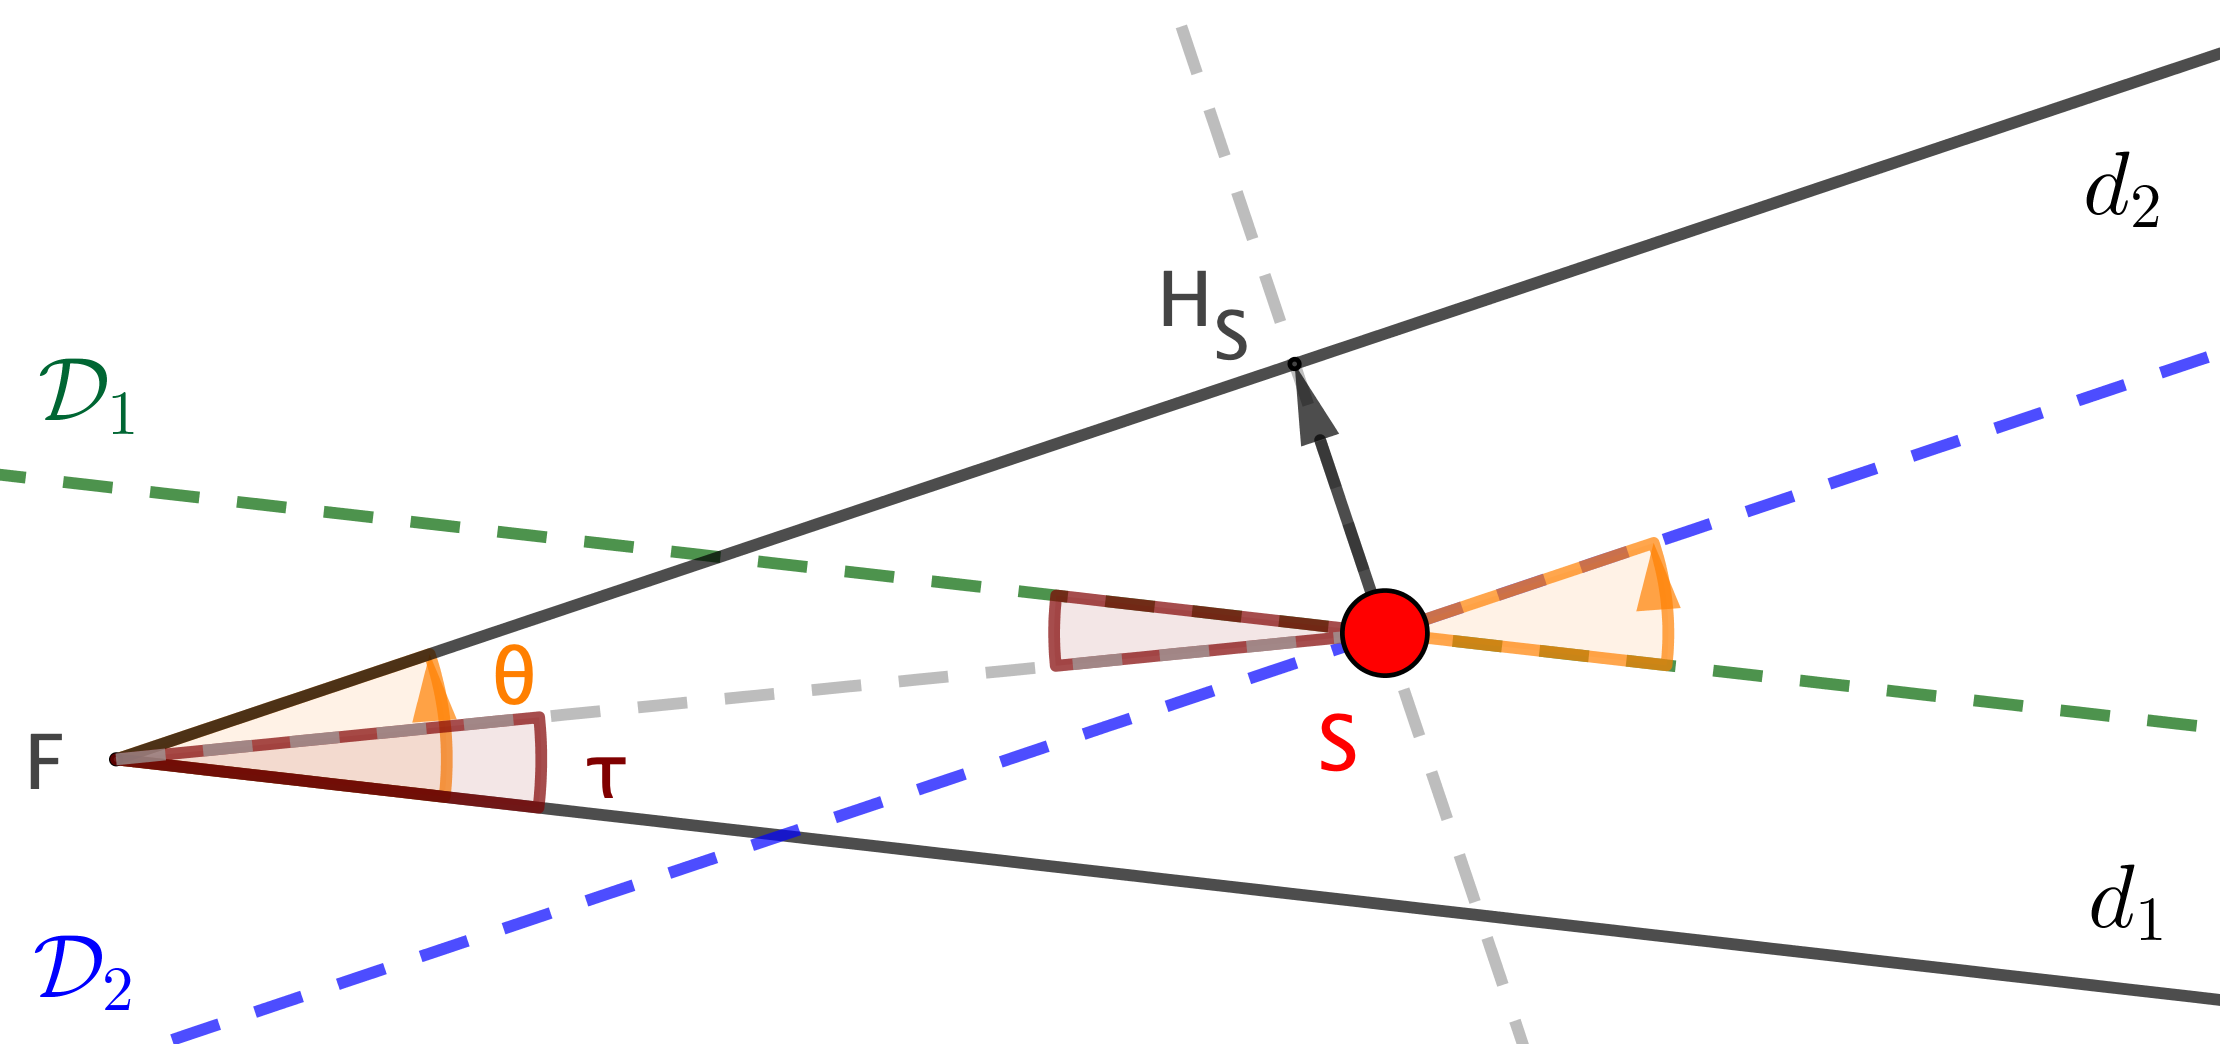
\includegraphics[width=12cm]{content/proof-1st-bounce-somewhere.png}

		\itshape\small
		Les autres cas
	\end{center}
\end{proof}


Il nous reste juste à traiter les cas d'un 1\ier{} rebond se faisant sur $\setgeo*{d}{1}$ et $\setgeo*{d}{2}$ respectivement.

\begin{tcolorbox}
	\centering\itshape
	
	En fait, nous n'avons besoin de traiter que la situation d'un 1\ier{} rebond sur $\setgeo*{d}{2}$.
\end{tcolorbox}

En effet, une fois ceci étudié, l'autre cas s'obtiendra avec le même type de raisonnement excepté que l'on projettera $S$ sur $\setgeo*{d}{1}$ au lieu de $\setgeo*{d}{2}$.



\section{Quand le 1\ier{} rebond se fait "vers le haut"}

\begin{fact} \label{ortho-rebond}
	Supposons que $\sigma_S = 0$.
	
	\medskip
	
	Notant $M$ l'intersection de $(SH_S)$ avec $\setgeo*{d}{1}$, nous avons que $M$ est sur le trajet de la bille avec $\sigma_M < 0$
	\footnote{
		On pourrait avoir un résultat plus fin mais ceci ne nous serait inutile pour la suite.
	}.
\end{fact}

\begin{proof}
	Évident grâce au dessin précédent.
\end{proof}


\medskip


\begin{fact} \label{deux-rebonds-vers-F}
	Supposons que $\sigma_S \in \intervalO{0}{\dfrac{\pi}{2} - \theta + \tau}$.
	
	\medskip
	
	Il existe un point $M$ sur le trajet de la bille, mais pas sur $\setgeo*{d}{1}$, tel que $\sigma_M  < 0$.
\end{fact}

\begin{proof}
	Au bout de deux rebonds, nous avons trois situations possibles dont les deux premières ci-après ne nécessitent aucune explication.
	
	
	\medskip
	
	\begin{center}
		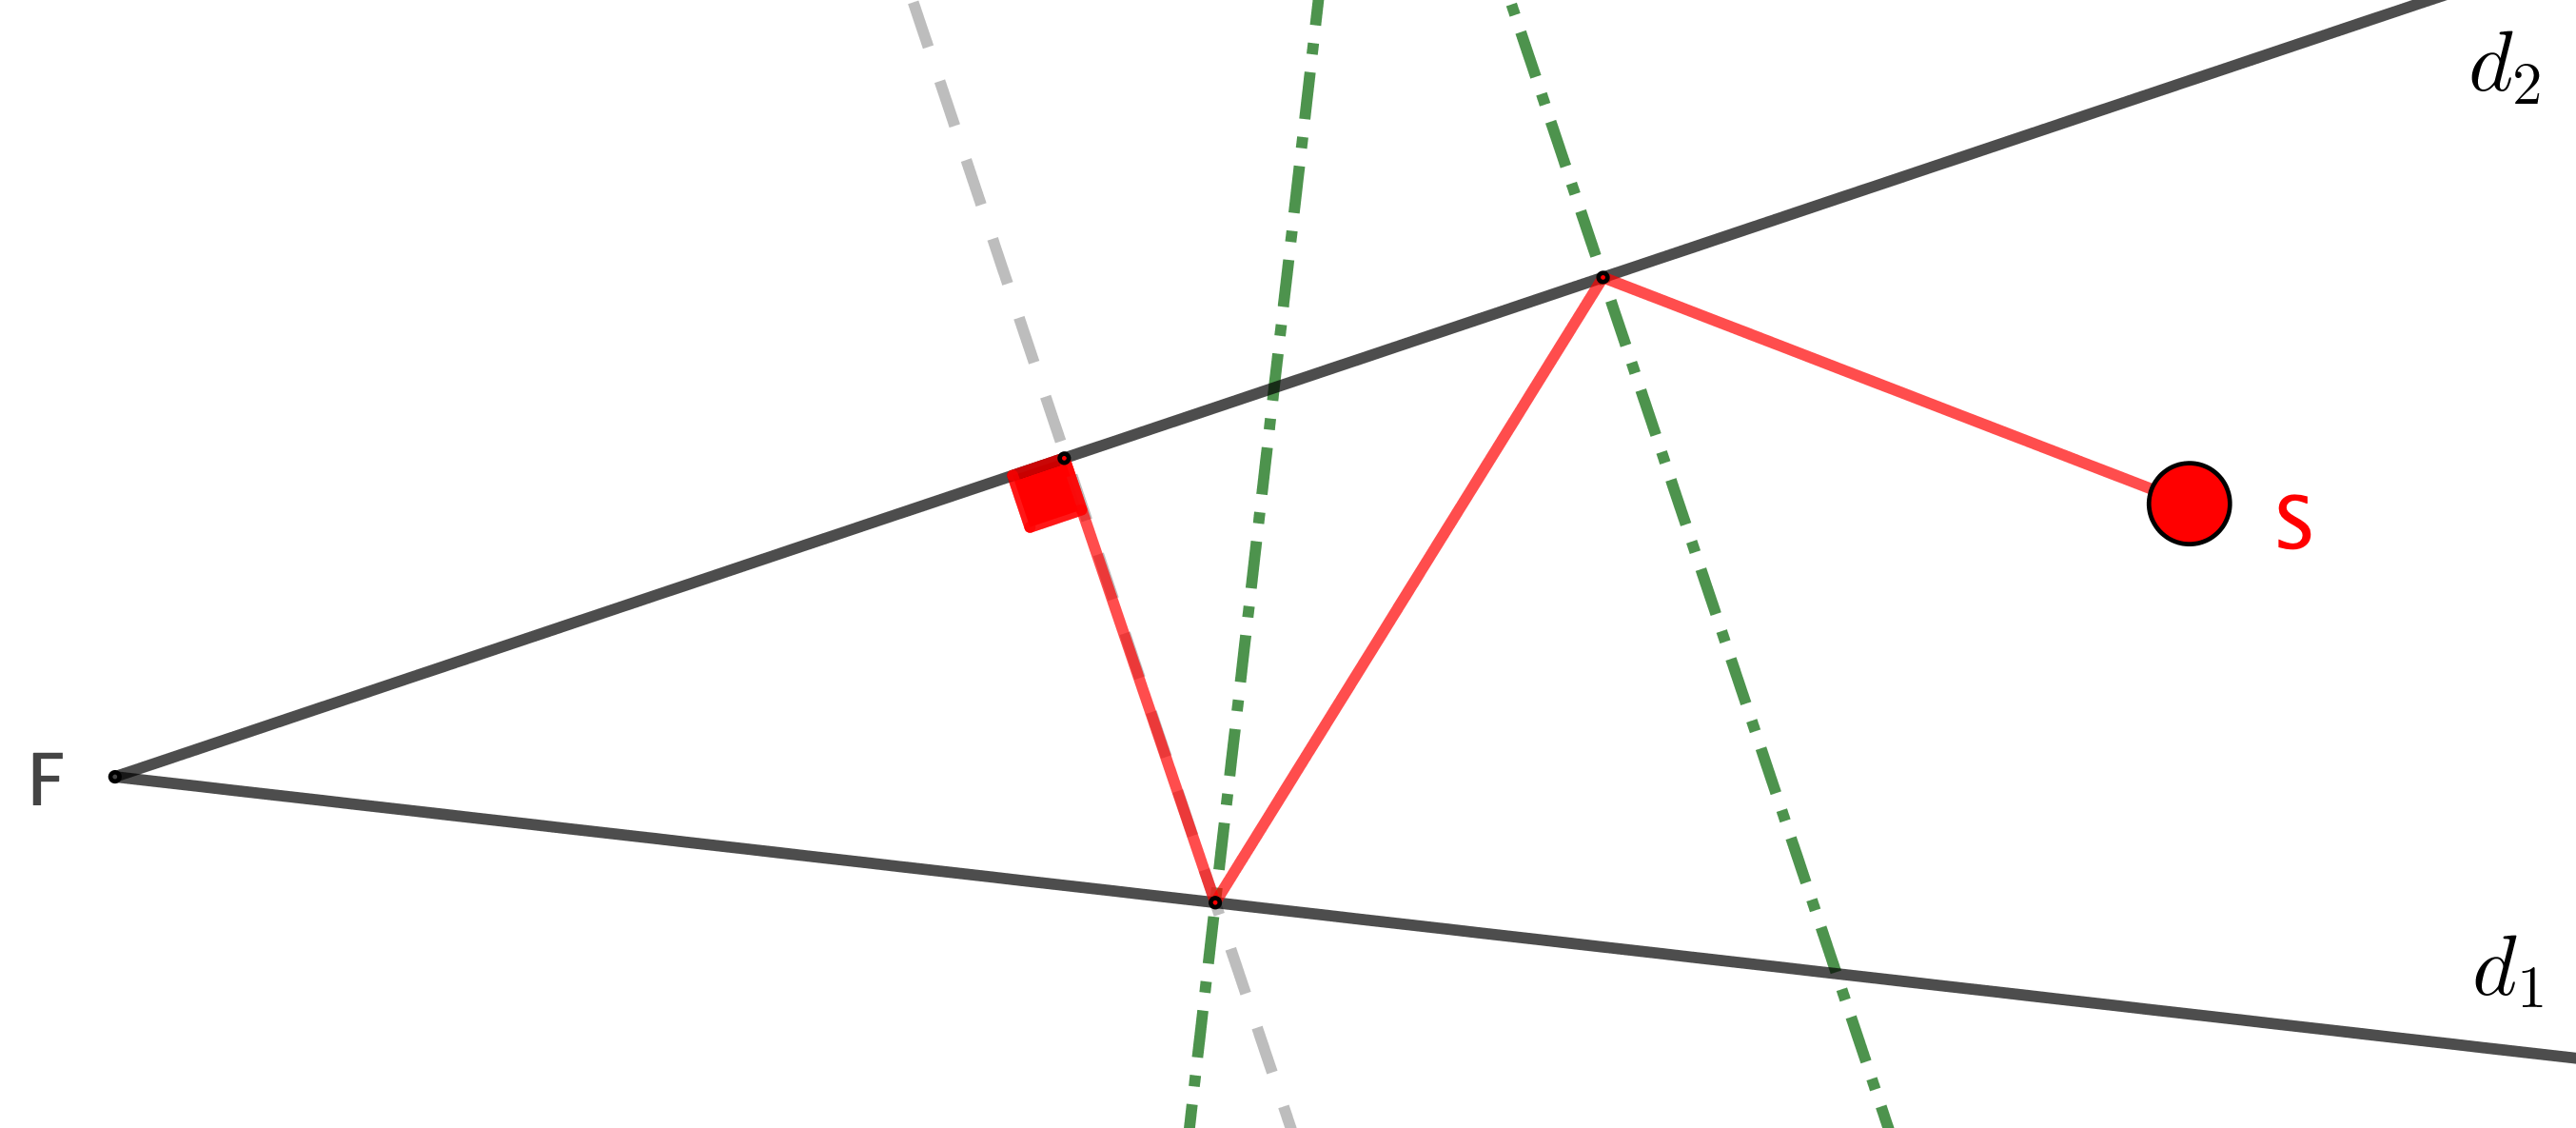
\includegraphics[width=12cm]{basic-math-pool/proof-starting-with-d2-2-bounces-to-ortho.png}

		\itshape\small
		Le 2\ieme{} rebond nous ramène à la situation du fait \ref{ortho-rebond} ci-dessus
		
		qui nous permet de conclure directement.
	\end{center}
	
	
	\medskip
	
	\begin{center}
		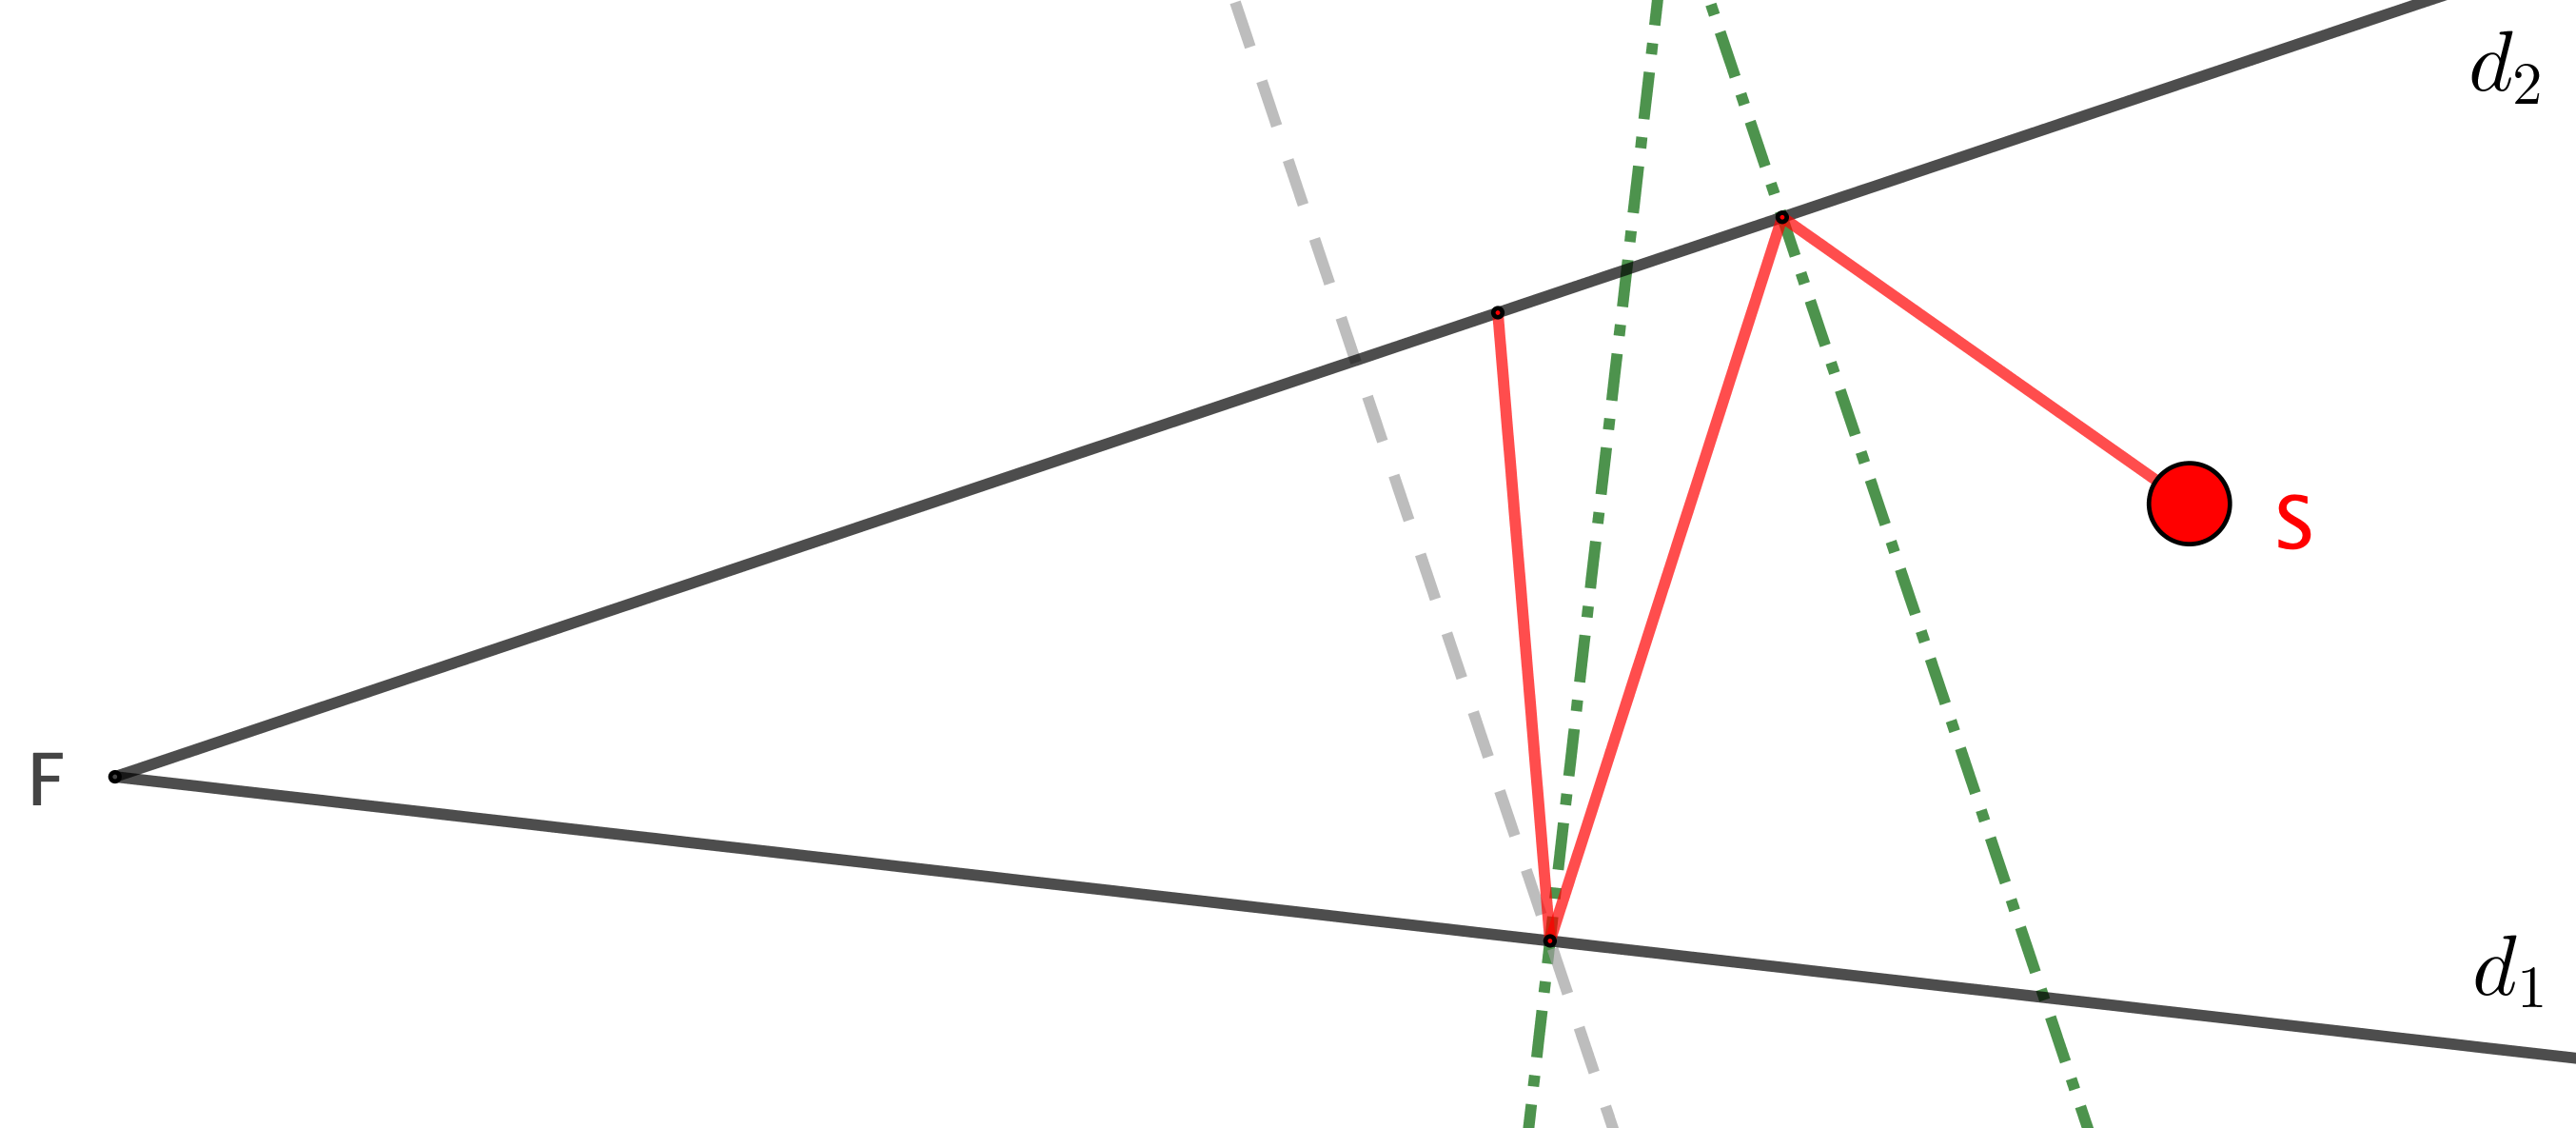
\includegraphics[width=12cm]{basic-math-pool/proof-starting-with-d2-2-bounces-to-infinity.png}

		\itshape\small
		Le 2\ieme{} rebond nous ramène directement à la bonne situation.
	\end{center}
	
	
	\medskip
	
	Voici la dernière situation représentée ci-dessous où $\setgeo{D}_2 \, /\!/ \, \setgeo{d}_2$.
	
	
	\medskip
	
	\begin{center}
		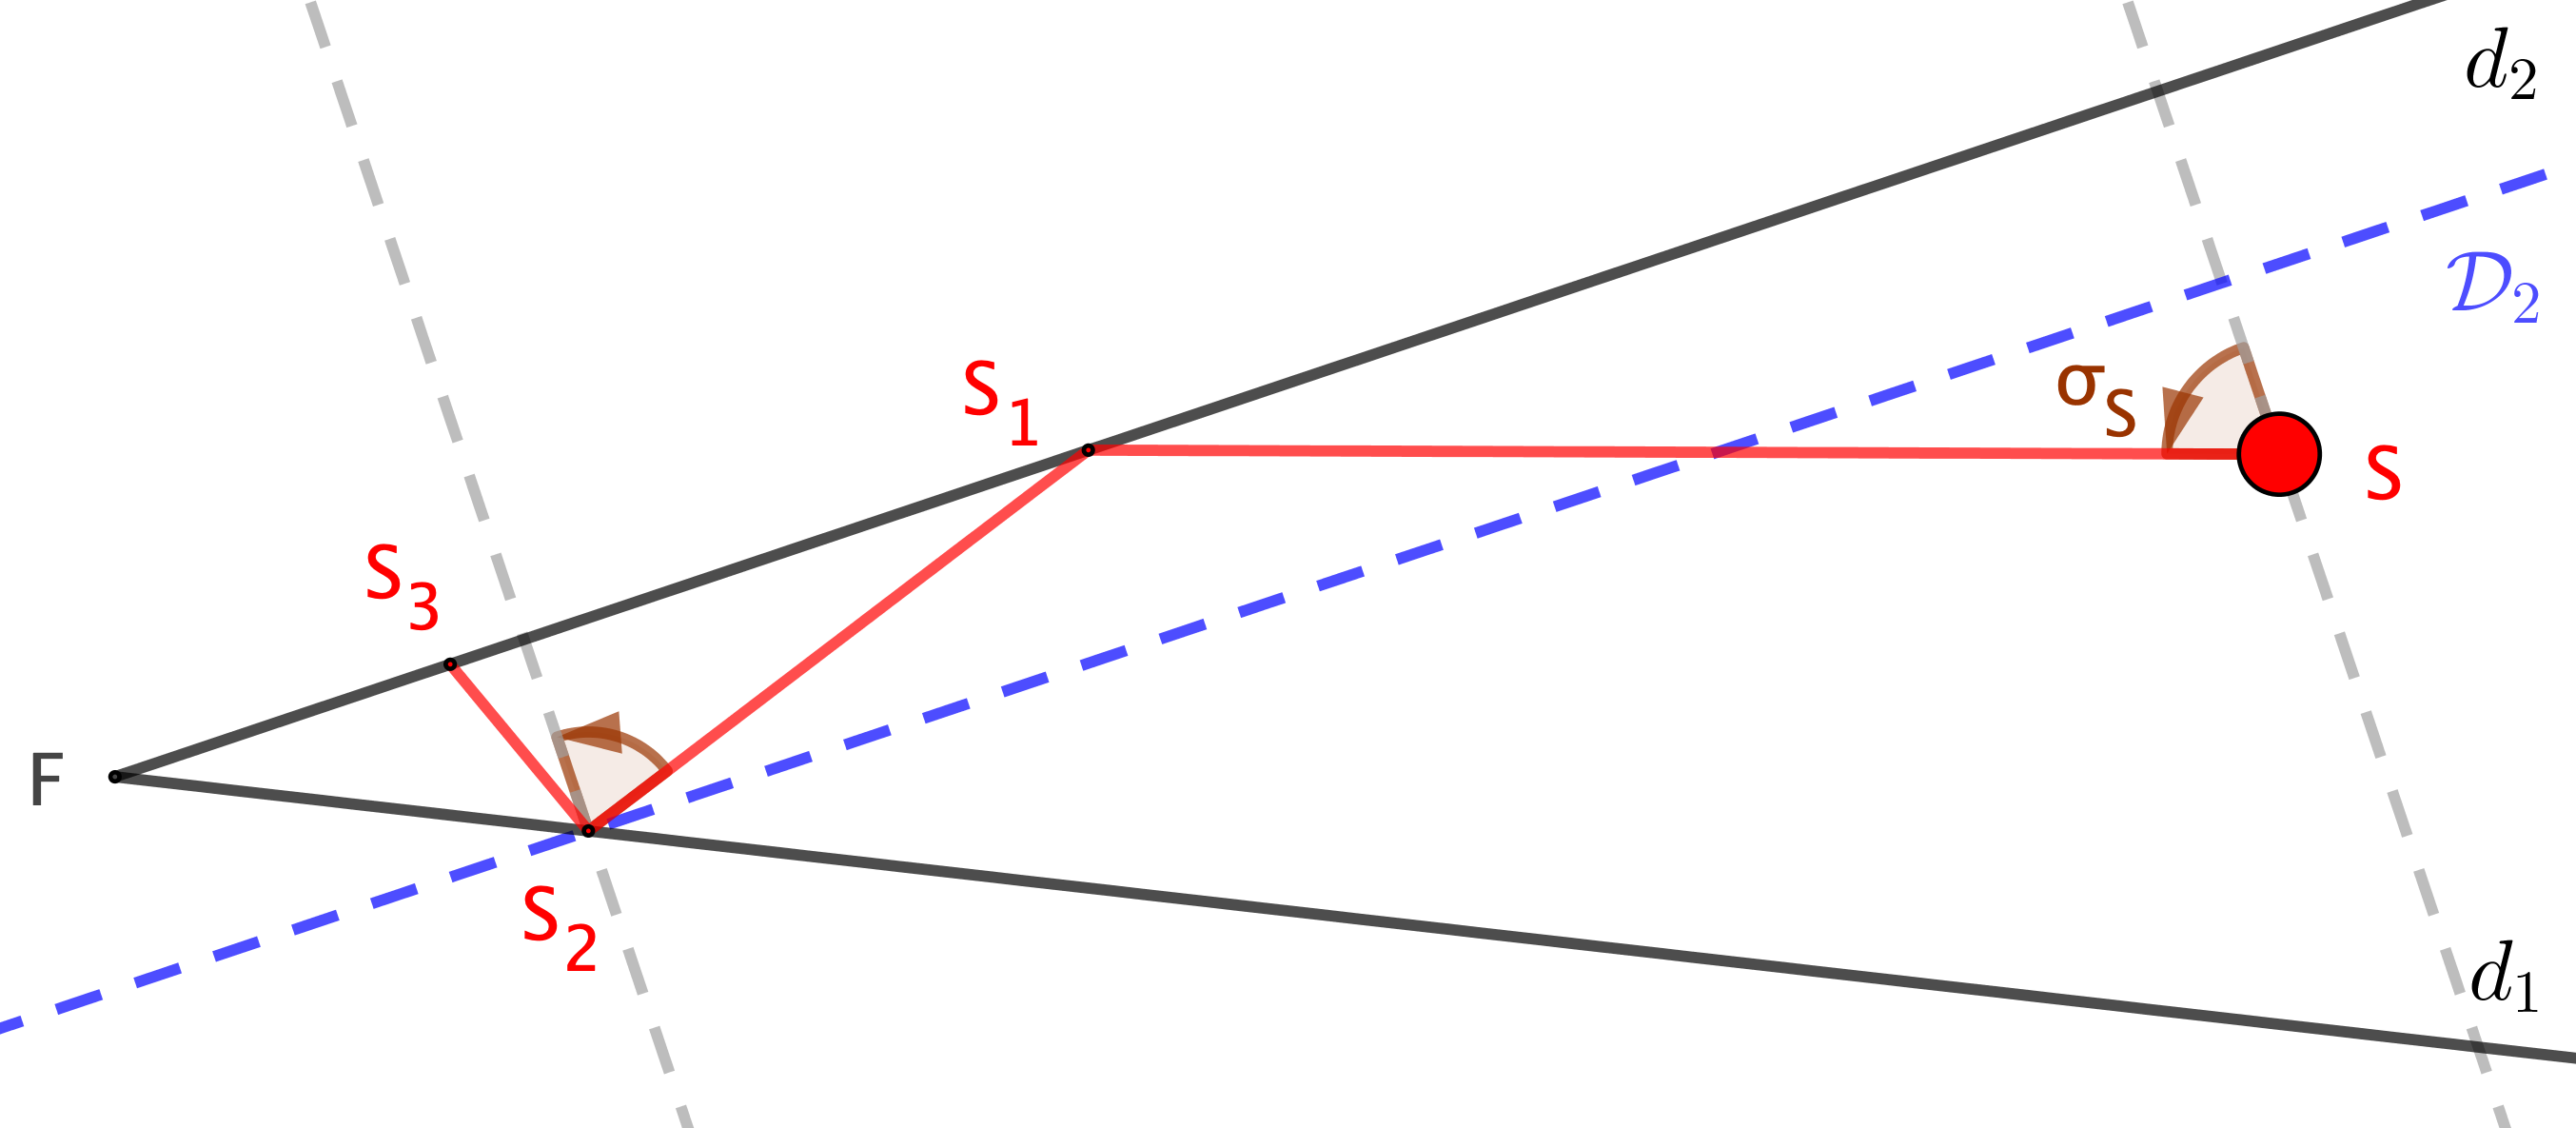
\includegraphics[width=12cm]{basic-math-pool/proof-starting-with-d2-2-bounces-to-F.png}

		\itshape\small
		Le 2\ieme{} rebond nous ramène à la situation de départ
		
		mais avec une valeur de $\sigma$ qui a augmenté.
	\end{center}
	
	
	\medskip
	
	Faisons un zoom sur la partie de gauche pour évaluer précisément l'évolution faisant passer de $\sigma_S$ à $\sigma_{S_2}$.
	
	\begin{center}
		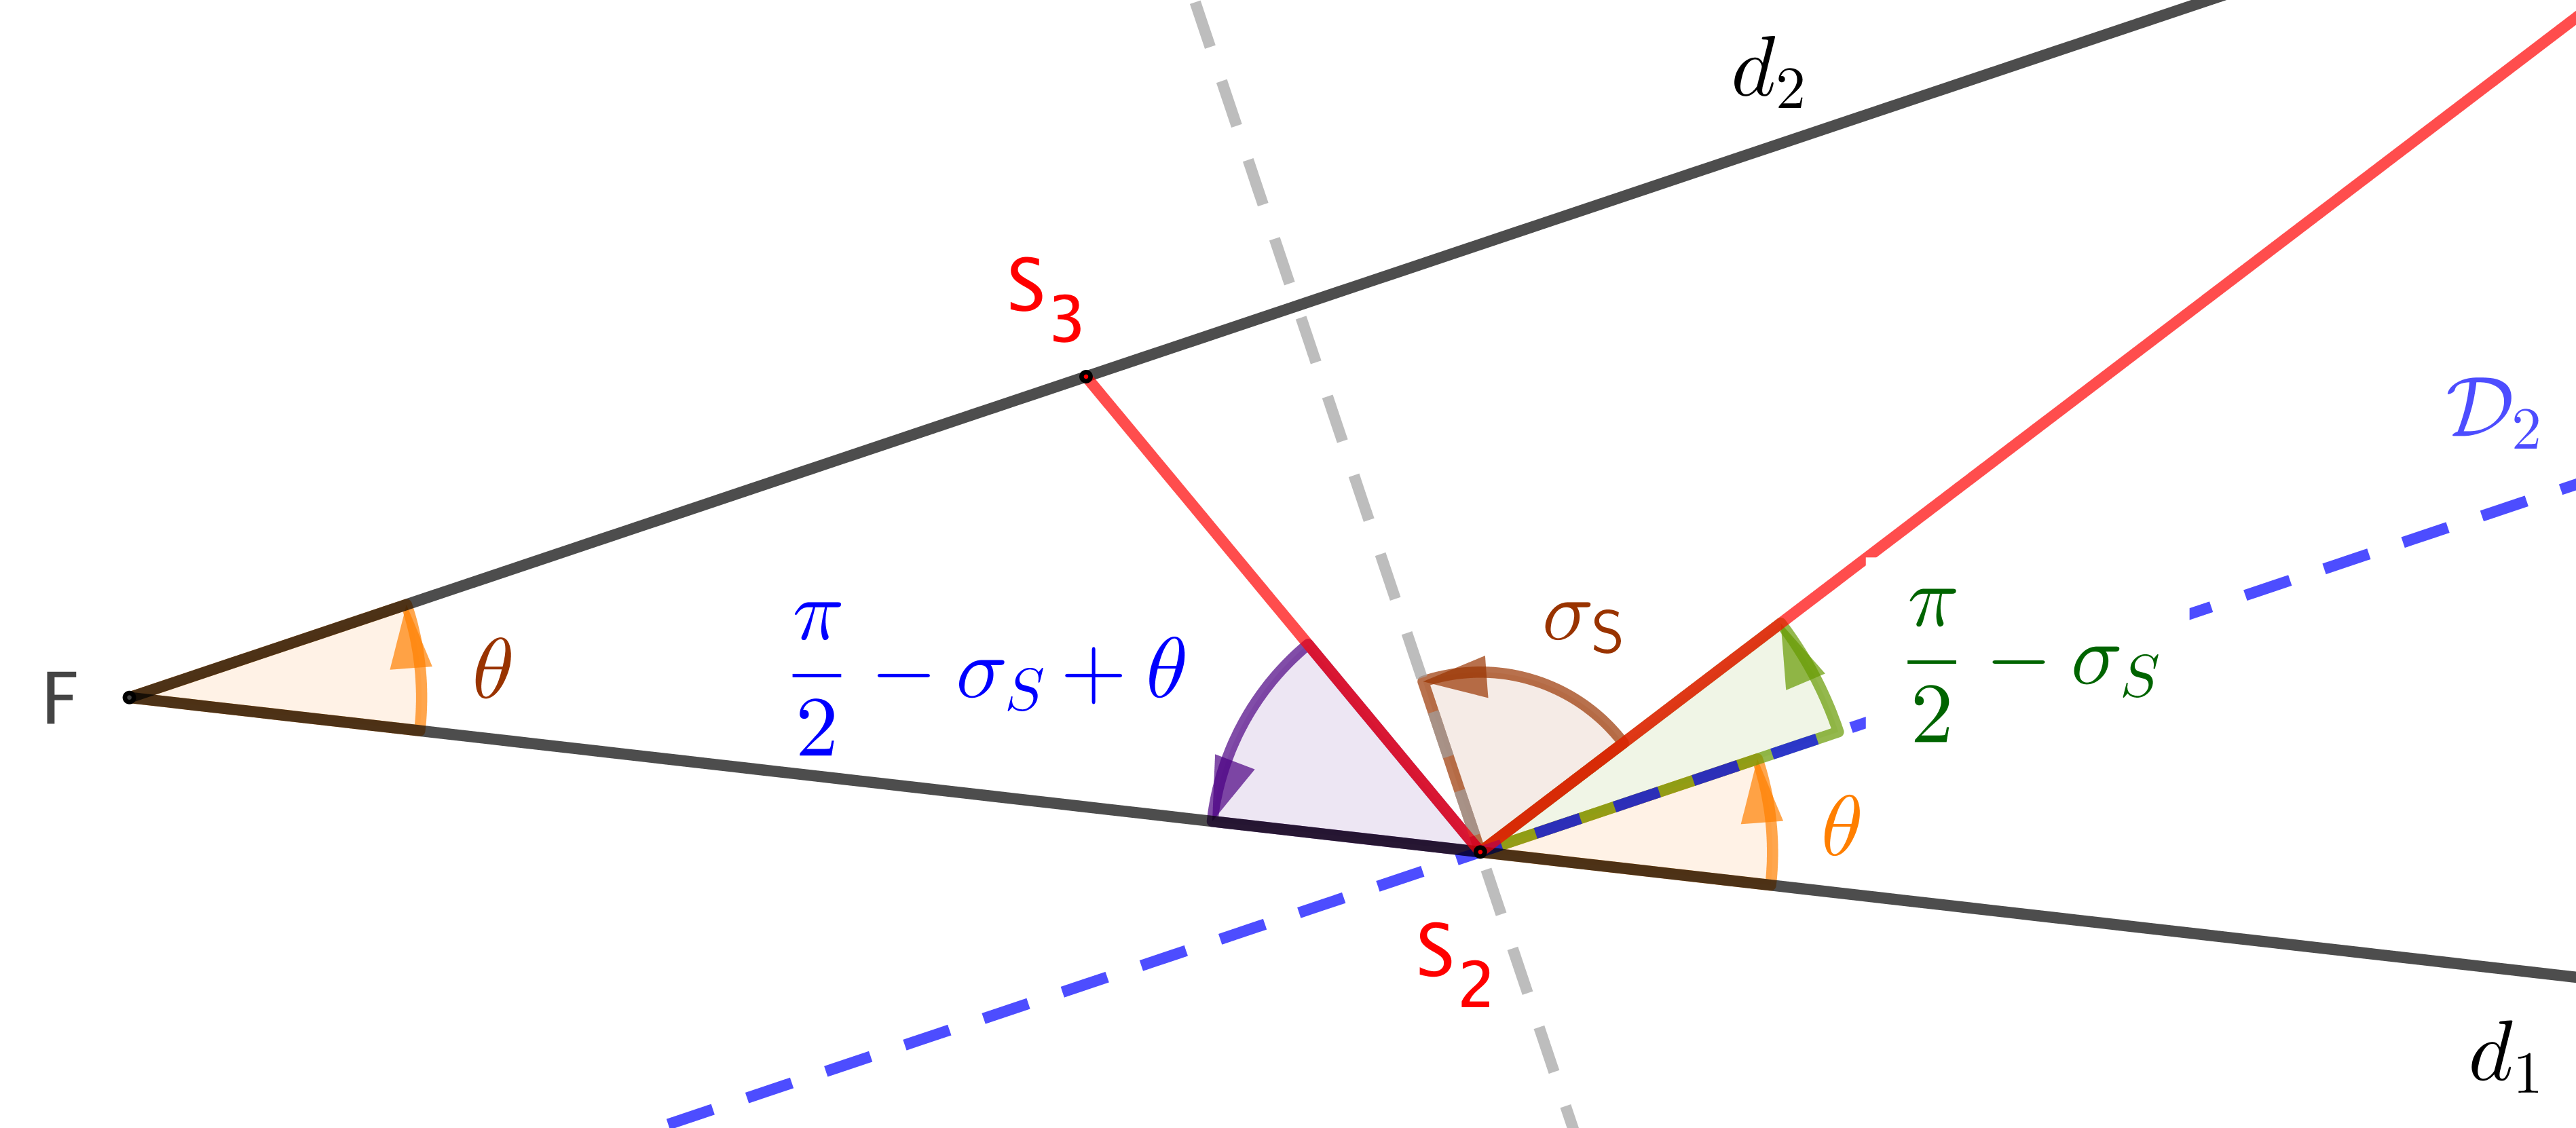
\includegraphics[width=12cm]{basic-math-pool/proof-starting-with-d2-2-bounces-to-F-zoom.png}
	\end{center}
	
	
	\medskip
	
	Nous avons alors $\sigma_{S_2} = \pi - 2 \left( \dfrac{\pi}{2} - \sigma_S + \theta \right) - \sigma_S = \sigma_S - 2 \theta$.
	Ceci montre que l'on passe de $\sigma_S$ à $\sigma_{S_2} = \sigma_S + \delta$ où $\delta = - 2 \theta < 0$. Cette dernière relation montre que l'on ne pourra pas avoir indéfiniment la dernière situation \emph{(en toute rigueur, il faudrait faire un raisonnement par récurrence)}.  
\end{proof}


\medskip


\begin{fact} \label{s-eloigner}
	Supposons que $\sigma_S \in \intervalCO{- \dfrac{\pi}{2}}{0}$.

	\medskip
	
	Il existe un point $M$ sur le trajet de la bille, mais pas sur $\setgeo*{d}{1}$, tel que $\sigma_M < - \dfrac{\pi}{2}$. En particulier, à partir de ce point $M$ la bille s'éloignera indéfiniment loin de $F$.
\end{fact}

\begin{proof}
	La démarche est similaire à la preuve précédente.
	Pour la situation problématique, on utilise les deux graphiques donnés dans la page suivante qui nous montrent que l'on passe de $\sigma_S$ à $\sigma_{S_2} = \sigma_S + \delta$ où $\delta = - 2 \theta < 0$. Ceci nous permet une seconde fois de conclure puisque l'on ne pourra pas avoir indéfiniment $\sigma_{S_{2k}} \geqslant - \dfrac{\pi}{2}$.
\end{proof}


\medskip


\begin{theorem}
	Si le 1\ier{} rebond se fait sur $\setgeo*{d}{2}$ alors il n'y aura qu'un nombre fini de rebonds et le dernier rebond amènera la bille à s'éloigner indéfiniment loin de $F$.
\end{theorem}

\begin{proof}
	Distinguons trois cas.
	
	\begin{itemize}[label = \textbullet]
		\item Si $\sigma_S \in \intervalCO{- \dfrac{\pi}{2}}{0}$ alors tout est donné par le fait \ref{s-eloigner}.


		\item Si $\sigma_S = 0$ alors le fait \ref{ortho-rebond} nous donne un point $M$ sur le trajet de la bille, mais pas sur $\setgeo*{d}{1}$, tel que $\sigma_M < 0$.
		
		\noindent
		Si $\sigma_M < - \dfrac{\pi}{2}$, nous savons qu'à partir de $M$ la bille s'éloignera indéfiniment loin de $F$.
		
		\noindent
		Sinon nous avons $\sigma_M \in \intervalCO{- \dfrac{\pi}{2}}{0}$.
		Le fait \ref{s-eloigner} nous permet alors de conclure.
		
		
		\item Enfin si $\sigma_S \in \intervalO{0}{\dfrac{\pi}{2} - \theta + \tau}$, il suffit de raisonner comme dans le point précédent mais en invoquant le fait \ref{deux-rebonds-vers-F}.
	\end{itemize}
\end{proof}

	
\medskip


\begin{center}
	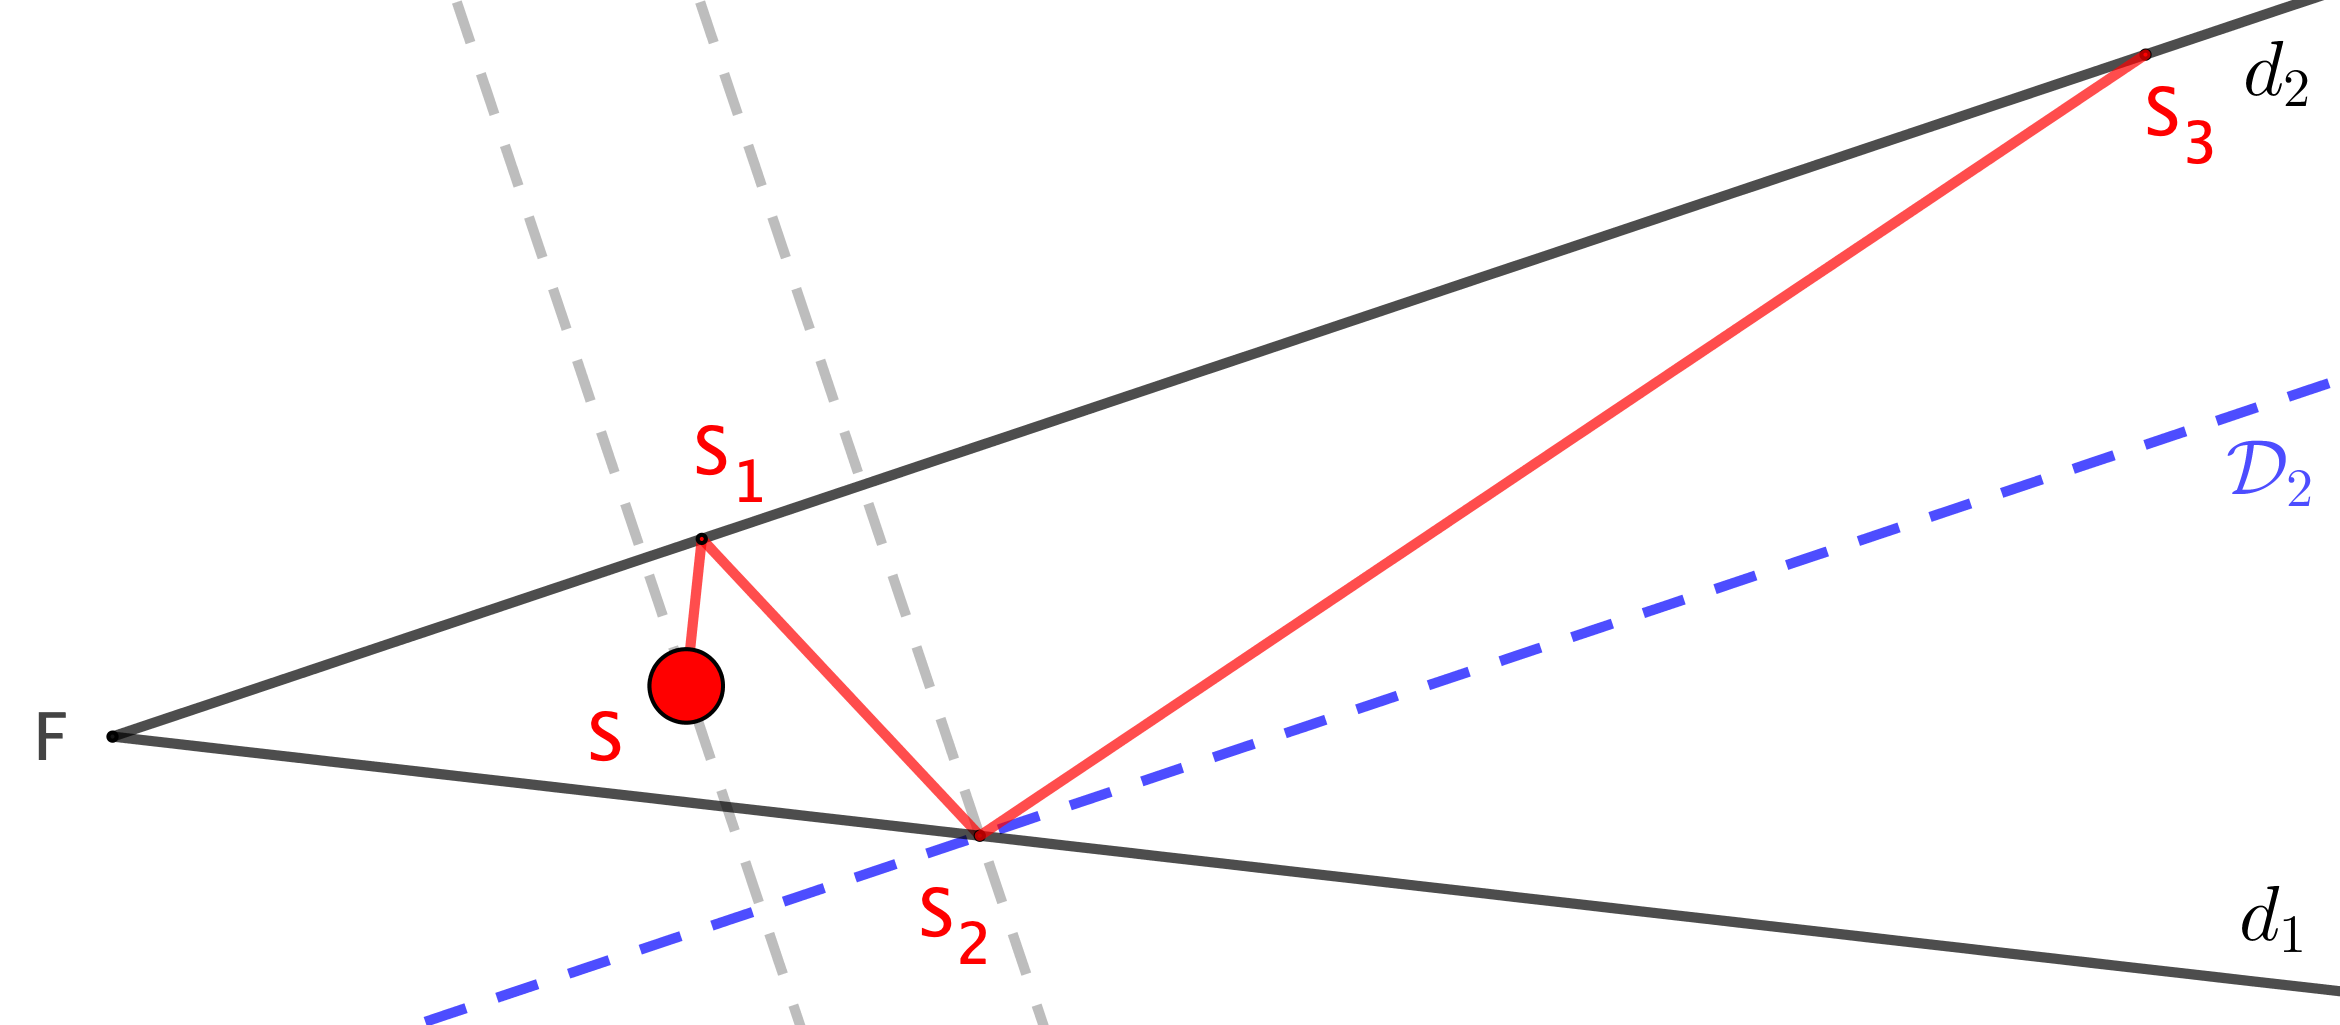
\includegraphics[width=12cm]{basic-math-pool/proof-starting-with-d2-2-bounces-farway-from-F.png}

	\itshape\small
	Preuve du fait \ref{s-eloigner} -- Vue large du cas problématique
\end{center}

	
\medskip


\begin{center}
	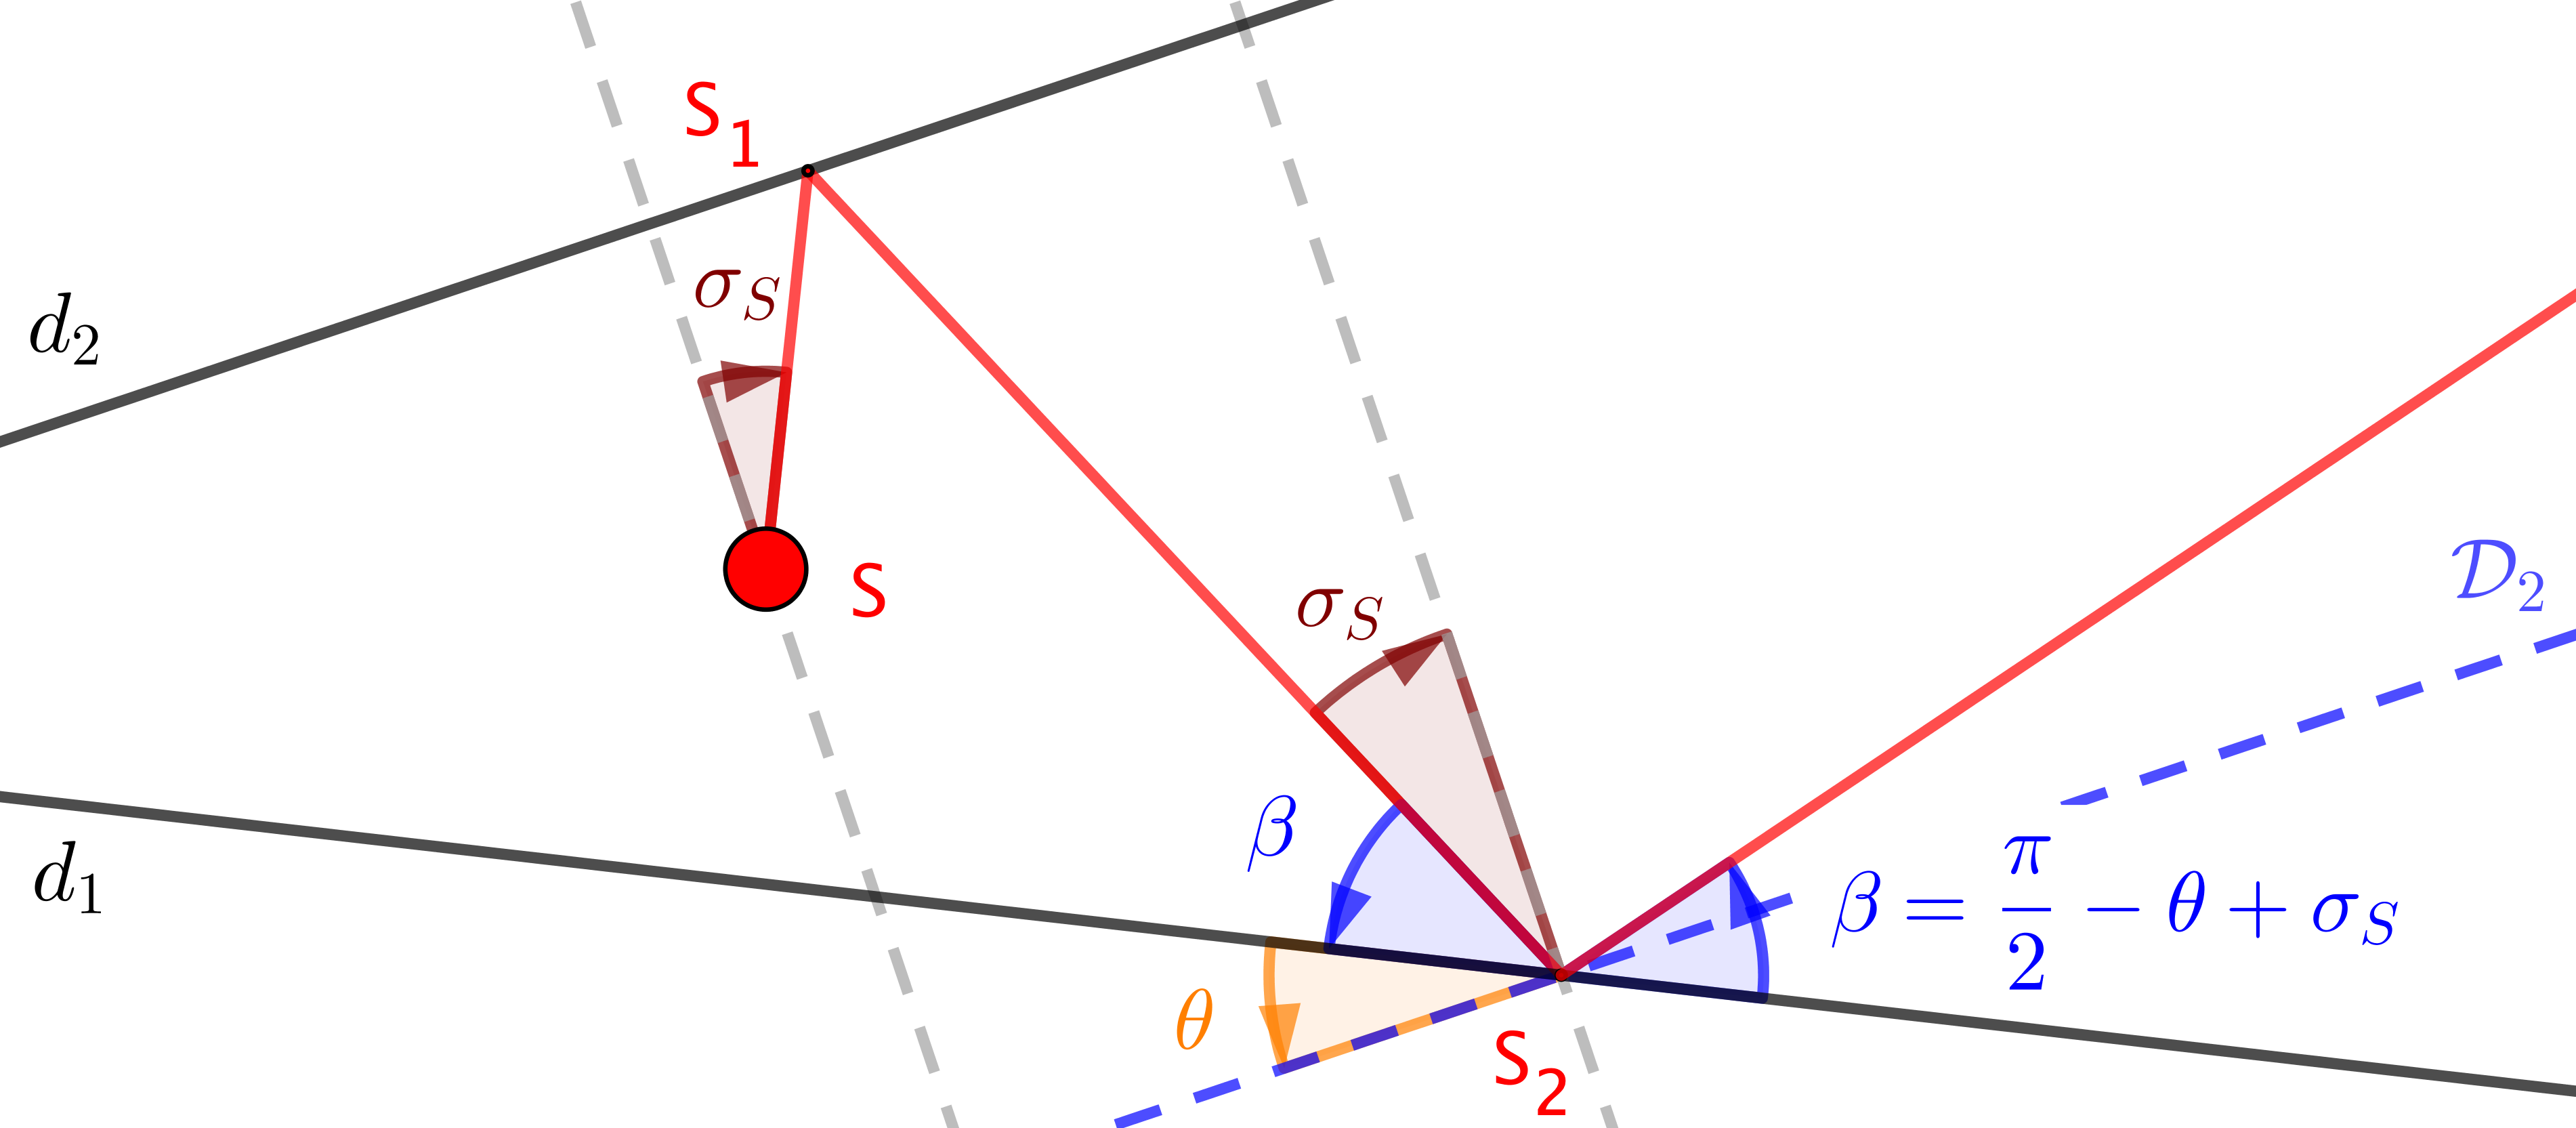
\includegraphics[width=12cm]{basic-math-pool/proof-starting-with-d2-2-bounces-farway-from-F-zoom.png}

	\itshape\small
	Preuve du fait \ref{s-eloigner} -- Vue zoomée du cas problématique
\end{center}



\end{document}
